\documentclass[a4paper]{cas-dc}

\usepackage{graphicx}
\graphicspath{{./}{figures/}}
\pdfcompresslevel=9
\pdfobjcompresslevel=3
\usepackage{amsmath,amssymb}
% expansion=false: cas-dc+STIX font expansion routinely exceeds Overleaf free compile time
\usepackage[protrusion=true,expansion=false,tracking=false,spacing=false,kerning=false]{microtype}
\usepackage{xcolor}
\usepackage{amsthm}
\theoremstyle{definition}
\newtheorem{definition}{Definition}
\usepackage{booktabs}
\usepackage{array}
\usepackage{tabularx}
\usepackage{multirow}
\usepackage{adjustbox}
\usepackage{subcaption}
\usepackage[justification=centering]{caption}
\renewcommand{\qedsymbol}{}
\usepackage{placeins}
\raggedbottom
\emergencystretch=2em
\tolerance=2000
\hbadness=10000
\vbadness=10000

% cas-dc packs ARTICLE INFO into \hbox to 0pt (intentional protrusion), always
% logging Overfull ~123.6pt. Re-wrap with \hss so TeX does not mark it overfull.
\ExplSyntaxOn
\RenewDocumentEnvironment { Abstract } { o }
{
  \group_begin:
  \IfNoValueTF { #1 } { }
  { \gdef\abstractname{#1} }
  \parindent = 0pt
  \box_if_empty:NTF \g_stm_key_box
  { \leftskip = .35 \textwidth }
  {
    \dim_gset:Nn \l_tmpa_dim { \box_ht:N \g_stm_key_box }
    \dim_gadd:Nn \l_tmpa_dim { \box_dp:N \g_stm_key_box }
    \leftskip = .35 \textwidth
    \hspace*{-.35 \textwidth }
    \noindent \hbox_to_wd:nn { 0pt } { \box_use_drop:N \g_stm_key_box \hss }
    \skip_vertical:n { -\l_tmpa_dim }
  }
  \noindent \abstractname \par
  \skip_vertical:n { -4pt }
  \noindent \rule{.65\textwidth}{.2pt} \par \footnotesize
  \ignorespaces \everypar { \parindent = 1.5em }
}
{ \par \group_end: }
\ExplSyntaxOff

\renewcommand{\topfraction}{0.95}
\renewcommand{\bottomfraction}{0.90}
\renewcommand{\textfraction}{0.05}
\renewcommand{\floatpagefraction}{0.75}
\renewcommand{\dbltopfraction}{0.95}
\renewcommand{\dblfloatpagefraction}{0.75}
\setcounter{topnumber}{5}
\setcounter{bottomnumber}{5}
\setcounter{totalnumber}{10}
\setcounter{dbltopnumber}{5}
\setlength{\textfloatsep}{10pt plus 2pt minus 2pt}
\setlength{\floatsep}{8pt plus 2pt minus 2pt}
\setlength{\intextsep}{8pt plus 2pt minus 2pt}
\setlength{\abovecaptionskip}{6pt}
\setlength{\belowcaptionskip}{4pt}

\usepackage[numbers,sort]{natbib}
\usepackage{url}
\usepackage{doi}

\newtheorem{theorem}{Theorem}
\newtheorem{proposition}{Proposition}
\newtheorem{corollary}{Corollary}
\newtheorem{remark}{Remark}
\usepackage{algorithm}
\usepackage{algorithmic}

\definecolor{myblue}{RGB}{0,0,150}
\hypersetup{
  colorlinks=true,
  linkcolor=myblue,
  citecolor=myblue,
  urlcolor=myblue,
  breaklinks=true
}

\makeatletter
\def\printorcid{}
\def\orcidID#1{}
\def\ORCID#1{}
\makeatother

\begin{document}

\shorttitle{CRC-GAD: Conformal Calibration for Graph Anomaly Scores}
\shortauthors{Khan et al.}


\title[mode=title]{CRC-GAD: Split-Conformal Calibration for Graph Anomaly Scores}

\author[1]{Amaan Ulla Khan}
\author[1]{Dr. Renu Dhir}
\author[1]{Indu Sounkhla}

\affiliation[1]{organization={Dr.\ B R Ambedkar National Institute of Technology},
    addressline={GT Road Amritsar Bypass},
    city={Jalandhar},
    postcode={144008},
    state={Punjab},
    country={India}}
\begin{abstract}
Unsupervised graph anomaly detectors produce useful node rankings, but converting those rankings into alerts at a user-chosen false-alarm budget remains unprincipled: raw score thresholds lack finite-sample meaning.
We present \textbf{CRC-GAD}, a backbone-agnostic \emph{split conformal calibration} layer for graph anomaly scores---\emph{not} a new GNN architecture and \emph{not} a new CoLA/DOMINANT variant.
Given any frozen scoring function, CRC-GAD draws a label-free random calibration--test partition of evaluation nodes and forms conformal p-values by ranking each test score against the calibration reference.
\textbf{What is guaranteed.} Theorem~\ref{thm:randomization} states that for a uniformly random test node, $\Pr(p_i \leq \alpha) \leq \alpha$ under the randomness of the partition alone---without requiring exchangeability of node scores.
This is a \emph{marginal, random-test-node} validity statement. It is \emph{not} a node-conditional FPR guarantee, and it is not automatically identical to the empirical false-positive rate among normal nodes.
\textbf{What transfers to normal-node FPR.} When anomalous scores stochastically dominate normal scores, the random-test-node bound implies a conservative bound on expected normal-node FPR; when the backbone inverts the ranking, that bridge can fail (Section~\ref{sec:th_limitations}).
We further derive a flagged-rate identity that makes every reported (FPR, TPR, anomaly fraction) triple auditable.
Experiments apply the \emph{same} wrapper to multiple scorers (PyTorch DOMINANT, a simplified CoLA-inspired contrastive scorer used only as one backbone, degree, and attribute baselines), expand heuristic comparisons beyond a single graph, and report contamination and degree-stratified diagnostics plus an organic rare-class proxy on Cora.
All numbers regenerate from commit-pinned code (\url{https://github.com/Amaanullakhan/CRC_GAD}).
\end{abstract}

\begin{keywords}
Graph anomaly detection\sep
Conformal prediction\sep
False positive rate control\sep
Attributed networks\sep
Distribution-free inference\sep
Post-hoc score calibration
\end{keywords}

\begin{highlights}
\item CRC-GAD is a post-hoc split conformal wrapper, not a new detector.
\item Proven guarantee: marginal random-test-node validity, not conditional FPR.
\item Normal-node FPR needs a score-dominance bridge and can fail if ranking inverts.
\item Same wrapper validated on DOMINANT, CoLA-style, and heuristic scorers.
\item All tables regenerate from commit-pinned code.
\end{highlights}

\maketitle

\section{Introduction}
\label{sec:introduction}

Detecting anomalous nodes on attributed graphs is a vital task for organizations that must protect networked systems against abuse, fraud, and structural manipulation.
Applications span cybersecurity~\cite{ding2019dominant}, financial monitoring~\cite{xu2022conad}, social-media integrity~\cite{fan2020anomalydae}, telecom analytics~\cite{ma2021comprehensive}, and biomedical graph mining~\cite{akoglu2015graph}.
In deployed screening pipelines, such detectors act as automated filters whose alerts trigger downstream human review, so the reliability of each alert---not only its ranking---determines practical value~\cite{ma2021comprehensive,bates2023testing}.
Related deep GAD and multi-view detectors continue to improve ranking quality on attributed networks~\cite{shao2023kbsgdae,kong2025kbsdegad,gusare2026kbsmaf,shi2023kbsmutant,ge2024kbsestcn}.
The graph setting is challenging: node features and topology are tightly coupled, normality is contextual, and anomaly labels are rarely available at scale~\cite{ma2021comprehensive}.
Traditionally, anomaly detection on graphs relied on hand-crafted ego-network statistics, community residuals, and spectral features~\cite{akoglu2015graph,sen2008collective}.
These methods remain interpretable but often fall short on large attributed networks where nonlinear interactions between structure and high-dimensional attributes dominate.
With the advancement of deep learning, graph neural networks (GNNs)~\cite{kipf2017gcn,hamilton2017inductive,velickovic2018graph} have received much attention for unsupervised anomaly detection.
Reconstruction-based architectures~\cite{ding2019dominant,fan2020anomalydae,yuan2021guide} learn to encode and decode the graph, treating large reconstruction errors as anomaly signals.
Complementarily, contrastive self-supervision~\cite{chen2020simclr,oord2018representation} trains encoders by contrasting nodes against local subgraph context; representative graph anomaly detectors include subgraph-level instance discrimination~\cite{liu2022cola}, multi-view contrastive designs~\cite{zheng2021slgad,jin2021anemone,xu2022conad}, and recent robustness-oriented extensions~\cite{luo2025adgcl,shi2025cvgad,qiao2025uniform}.
Across these families, modern unsupervised scorers typically produce a real-valued anomaly ranking without access to ground-truth labels during training.

However, applying deep graph anomaly scorers in operational settings still faces obstacles that are largely orthogonal to raw ranking accuracy.
Based on our setting and related literature~\cite{ma2021comprehensive,bates2023testing}, we summarize two major limitations:
\begin{enumerate}
  \item \textbf{Uncalibrated decision statistics.} Raw scores lack a transparent mapping from numerical value to operational risk; practitioners often tune thresholds by trial and error, validation heuristics, or rules of thumb that are hard to justify to auditors or safety reviewers.
  \item \textbf{Lack of finite-sample, distribution-free error control.} Standard post hoc thresholds do not generally yield a provable bound on the false positive rate among normal entities at a user-chosen nominal level---precisely the form of guarantee increasingly expected in anti--money laundering workflows~\cite{bates2023testing}, clinical alerting, and intrusion analytics.
\end{enumerate}

To address these challenges, we present \textbf{CRC-GAD} (\textbf{C}onformal \textbf{R}isk-\textbf{C}ontrolled \textbf{G}raph \textbf{A}nomaly \textbf{D}etection), a lightweight \emph{post-hoc calibration} framework that wraps a \emph{frozen} score-based graph anomaly detector with split inductive conformal prediction~\cite{vovk2005algorithmic,papadopoulos2002inductive,angelopoulos2023conformal}.
\textbf{Scope of novelty.} CRC-GAD does \emph{not} introduce a new graph neural architecture, does not modify CoLA~\cite{liu2022cola} or DOMINANT~\cite{ding2019dominant}, and does not claim higher AUC than existing scorers.
Its contribution is the calibration protocol: converting any fixed score vector into conformal p-values with a precisely stated marginal guarantee under a label-free random partition (Section~\ref{sec:prob_fpr}).
CRC-GAD never changes the backbone architecture and requires no anomaly labels at calibration time: it consumes the scorer's outputs only.

Conformal prediction maps arbitrary nonconformity scores to calibrated significance measures.
In the split (inductive) formulation, each test score is ranked against a held-out calibration reference, yielding a p-value that satisfies $\Pr(p \leq \alpha) \leq \alpha$ at any nominal level $\alpha \in [0,1]$ under standard exchangeability~\cite{angelopoulos2023conformal}; Section~\ref{sec:prob_fpr} states the construction used in CRC-GAD.
Our graph setting emphasizes validity induced by random partitioning of evaluation nodes (Theorem~\ref{thm:randomization} in Section~\ref{sec:theory}).
Although conformal methods have been applied to classification~\cite{romano2020classification}, regression~\cite{romano2019conformalized}, outlier testing~\cite{bates2023testing}, and select graph tasks~\cite{huang2024uncertainty,liu2024conformal}, \emph{post-hoc} unsupervised calibration of node-level graph anomaly scores under a label-free random partition remains underexplored---the gap CRC-GAD targets (orthogonal to designing a stronger scorer).

Specifically, CRC-GAD proceeds as follows:
\begin{enumerate}
  \item \textbf{Unsupervised scoring (any backbone).} Obtain frozen node anomaly scores $\{s_i\}$ from any score-based detector. For the primary tables we use a simplified CoLA-inspired contrastive scorer~\cite{liu2022cola}; Table~\ref{tab:backbones} also wraps PyTorch DOMINANT and heuristic scorers with the \emph{identical} conformal layer.
  \item \textbf{Random partition.} Split evaluation nodes, without using scores or labels, into a calibration set $\mathcal{C}$ and a test set $\mathcal{T}$ (Section~\ref{sec:prob_fpr}).
  \item \textbf{Conformal p-values.} For each $i \in \mathcal{T}$, assign $p_i$ by ranking $s_i$ against $\{s_j\}_{j \in \mathcal{C}}$ as in Eq.~\eqref{eq:pvalue_formal}.
  \item \textbf{Decision.} Flag $i$ if $p_i \leq \alpha$ for user-chosen $\alpha$.
\end{enumerate}
The procedure is non-invasive (no retraining of the scorer on calibration data, no labels for the $\mathcal{C}/\mathcal{T}$ split) and model-agnostic: CoLA-style and DOMINANT scores are interchangeable inputs to the same wrapper~\cite{ding2019dominant,fan2020anomalydae,xu2022conad}.

The main contributions of this paper are as follows:
\begin{enumerate}
  \item We formalize the \emph{calibration gap} in unsupervised graph anomaly detection and cast false-positive budgeting as a split conformal inference problem on graph-structured scores, so an operator can specify a nominal alarm level $\alpha$ instead of an uninterpretable score threshold.
  \item We establish \emph{random-test-node} validity under random calibration--test partitioning (Theorem~\ref{thm:randomization}), carefully distinguishing it from normal-node FPR and from node-conditional guarantees.
  \item We derive the flagged-rate identity (Proposition~\ref{prop:flagged}) and the contamination bias direction, and we validate both empirically.
  \item We instantiate CRC-GAD on multiple backbones (PyTorch DOMINANT~\cite{ding2019dominant}, a simplified CoLA-inspired contrastive scorer as one option, degree, and attribute baselines), expand heuristic comparisons beyond Cora, report degree-stratified FPR and runtimes, and include an organic rare-class proxy experiment (Sections~\ref{sec:exp_conformal_compare}--\ref{sec:abl_contamination}).
\end{enumerate}
Section~\ref{sec:related} reviews related work; Section~\ref{sec:problem}--\ref{sec:method} formalize the problem and CRC-GAD; Section~\ref{sec:experiments} reports experiments; Section~\ref{sec:conclusion} concludes.

\section{Related Work}
\label{sec:related}

We position CRC-GAD against three literatures: deep unsupervised GAD (strong ranking, uncalibrated thresholds), contrastive scorers (same gap), and conformal methods on graphs (mostly supervised coverage or tabular outliers).
\textbf{What is new.} Not a new GNN and not a new conformal statistic; a \emph{deployment protocol} that (i)~calibrates unsupervised node anomaly scores with a label-free random partition, (ii)~states the guarantee as marginal random-test-node validity rather than exchangeability of GNN scores, and (iii)~makes reported FPR/TPR triples auditable via the flagged-rate identity.
\textbf{What is not claimed.} We do not claim to outperform CoLA or DOMINANT on AUC; those methods supply scores, CRC-GAD supplies calibrated decisions.
Empirically the wrapper is reusable across contrastive, reconstruction (PyTorch DOMINANT), and structural/attribute scorers.

\subsection{Deep Graph Anomaly Detection}
\label{sec:rw_gad}

Anomaly detection on attributed networks aims to identify nodes whose structural or attribute-level patterns deviate from the network norm.  Classical approaches relied on hand-crafted features extracted from ego-networks, community residuals, or spectral projections of the graph Laplacian~\cite{akoglu2015graph,sen2008collective}.  While interpretable, these methods scale poorly and cannot capture the nonlinear entanglement between topology and high-dimensional attributes that characterizes modern networks.
The introduction of graph neural networks (GNNs)~\cite{kipf2017gcn,hamilton2017inductive,velickovic2018graph} enabled a new generation of deep anomaly detectors.  DOMINANT~\cite{ding2019dominant} established the reconstruction-based paradigm by coupling a GCN encoder with dual decoders that reconstruct the adjacency matrix and node feature matrix; nodes incurring large reconstruction errors under both decoders are flagged as anomalous.  AnomalyDAE~\cite{fan2020anomalydae} refined this idea with a dual-autoencoder architecture incorporating a cross-modal attention mechanism that allows the structure and attribute channels to share information through learned attention weights, improving detection of attribute-centric anomalies.  GUIDE~\cite{yuan2021guide} moved beyond first-order neighborhoods by using higher-order node motif degrees as input to a structure-aware autoencoder, capturing meso-scale patterns that first-order GCNs miss.  Shao et al.~\cite{shao2023kbsgdae} proposed a graph deep autoencoder that jointly reconstructs both structure and multiple attribute views for anomaly detection in multi-attributed networks.  GAAN~\cite{chen2020gaan} adopted a generative adversarial framework~\cite{goodfellow2014generative} in which a generator synthesizes fake attribute vectors and a discriminator learns to separate real from fake nodes, with the anomaly score combining reconstruction error and discriminator confidence.
GCN-based architectures have also been applied to anomaly detection beyond attributed networks; for instance, Shi et al.~\cite{shi2023kbsmutant} combined temporal GCNs with an attention-based variational autoencoder for multivariate time-series anomaly detection, and Ge et al.~\cite{ge2024kbsestcn} introduced an enhanced spatio-temporal constraints network that employs graph contrastive learning to capture inter-feature associations for anomaly detection.

Despite their empirical success, reconstruction-based and generative methods share two limitations.  First, they assume that anomalous nodes are poorly reconstructed by a model trained on the entire graph, an assumption that can fail when anomalies form tight clusters with internally consistent structure.  Second, they typically require full-graph decoding during both training and inference, which limits scalability to networks with hundreds of thousands of nodes.  Third, and most relevant to CRC-GAD, they output reconstruction errors or discriminator scores that are useful for ranking but are not accompanied by finite-sample, distribution-free guarantees on the false positive rate at a user-chosen significance level $\alpha$---precisely the operational requirement formalized in our contribution~(1).  These limitations motivated the development of contrastive approaches discussed next.
A number of recent surveys provide comprehensive overviews of the field.  Ma et al.~\cite{ma2021comprehensive} present a taxonomy of deep graph anomaly detectors organized by learning paradigm (reconstruction, contrastive, generative, and hybrid); broader treatments of anomaly detection include~\cite{chandola2009anomaly,chalapathy2017deep,ruff2020unifying}.  We refer the reader to these surveys for a broader landscape and focus here on the methods most relevant to our work.

\subsection{Contrastive Self-Supervised Methods}
\label{sec:rw_contrastive}

Contrastive self-supervised learning~\cite{chen2020simclr,oord2018representation} has emerged as a powerful alternative to reconstruction-based anomaly detection on graphs.  The central idea is to train an encoder that maps structurally or semantically similar instances close together in embedding space while pushing dissimilar instances apart, and then to use the degree of agreement (or disagreement) between a node and its context as the anomaly signal.

Liu et al.~\cite{liu2022cola} pioneered this direction by formulating anomaly detection as a subgraph-level instance discrimination task.  For each target node, the framework samples a local subgraph via random walks with restart~\cite{tong2006fast,perozzi2014deepwalk}, constructs positive pairs (node paired with its own subgraph) and negative pairs (node paired with foreign subgraphs), and trains a bilinear discriminator to distinguish the two.  Anomaly scores are obtained by averaging the positive--negative score gap over multiple independent sampling rounds.  Mini-batch training makes the approach scalable, and multi-round scoring provides implicit ensembling that stabilizes the output.  Published in IEEE TNNLS (2022), this line of work achieved strong performance on seven benchmark networks and has become a standard baseline.
Concurrent and subsequent work extended the contrastive paradigm in several directions.  {SL-GAD}~\cite{zheng2021slgad} combined a generative attribute regression module with a multi-view contrastive objective that constructs different contextual subgraphs around each target node, providing complementary views of both structural and attribute-level anomalies.  {ANEMONE}~\cite{jin2021anemone} introduced multi-scale contrastive learning that simultaneously measures agreement at both the patch (local) and context (global) levels, with a statistical estimator aggregating the multi-scale signals into a single anomaly score.  {CONAD}~\cite{xu2022conad} injected human priors about anomaly types through targeted graph augmentations-structural perturbation for structural anomalies, attribute noise for attribute anomalies-and trained a Siamese GNN with contrastive loss on original vs.\ augmented views.
More recent work has focused on robustness and fairness of contrastive anomaly detection.  {AD-GCL}~\cite{luo2025adgcl} identified a structural imbalance problem: nodes in the tail of the degree distribution are under-sampled during contrastive training, causing the detector to miss low-degree anomalies.  The method addresses this through neighbor pruning and anomaly-guided completion.  {CVGAD}~\cite{shi2025cvgad} observed that edges connecting normal and anomalous nodes introduce interference into the contrastive objective and proposed a progressive clean-view purification module.  {FewGAD}~\cite{zheng2024fewgad} explored the few-shot regime, where a handful of labeled anomalies are available, and proposed generative contrastive learning with high-order subgraph sampling to avoid augmentation-induced distortion.  {DE-GAD}~\cite{kong2025kbsdegad} combined diffusion-based graph enhancement with multi-view contrastive learning (node--node, node--subgraph, subgraph--subgraph) to improve the robustness and accuracy of graph anomaly detection.  {UniFORM}~\cite{qiao2025uniform} unified node-, edge-, and graph-level anomaly detection within a single self-supervised framework using energy-based GNNs and meta-learning.
Recent multi-modal approaches such as MAF~\cite{gusare2026kbsmaf} further improve detection by adaptively fusing structural, contextual, and latent representations to uncover camouflaged anomalies in attributed graphs.  Despite these advances in discriminative performance, a common limitation persists across the entire family: \emph{none of them provides calibrated anomaly scores with explicit marginal FPR semantics at a user-chosen $\alpha$}.  The raw contrastive scores are useful for ranking nodes but cannot be directly used for principled decision-making at a user-specified significance level $\alpha$ without ad hoc threshold tuning.  This limitation maps directly to contributions~(1)--(2): we keep scorers such as CoLA-style contrastive models and DOMINANT \emph{frozen} and wrap them with split conformal p-values satisfying $\Pr(p_i \leq \alpha) \leq \alpha$ marginally over a random calibration--test partition (Theorem~\ref{thm:randomization}), without redesigning their training objectives.  The end-to-end CRC-GAD pipeline is illustrated in Figure~\ref{fig:pipeline} (Section~\ref{sec:meth_overview}).
\subsection{Conformal Prediction and Its Application to Graphs}
\label{sec:rw_cp}

Conformal prediction (CP) is a distribution-free framework for constructing prediction sets or p-values with finite-sample validity guarantees.  Originally introduced by Vovk, Gammerman, and Shafer~\cite{vovk2005algorithmic} and popularized through accessible tutorials~\cite{angelopoulos2023conformal,shafer2008tutorial}, CP requires only that calibration and test examples be exchangeable-a condition strictly weaker than the i.i.d.\ assumption~\cite{lei2013conformal}.  The split (inductive) variant~\cite{papadopoulos2002inductive,lei2018distribution} is particularly practical: it partitions data into a training set (used to fit the model), a calibration set (used to compute nonconformity scores), and a test set (on which prediction sets or p-values are constructed), adding negligible computational overhead to any pre-trained model.
In the supervised learning setting, CP has been applied to classification~\cite{romano2020classification}, regression~\cite{romano2019conformalized}, and multiple testing with FDR control~\cite{bates2023testing,benjamini1995fdr}; related work has also explored uncertainty quantification for deep anomaly detection~\cite{zhang2024eswauncertainty}.  More broadly, conformal p-values have been used for outlier detection in tabular data, where the goal is to test whether a new observation belongs to the same distribution as the reference (calibration) set~\cite{bates2023testing}.
Within the graph learning community, interest in conformal methods has grown rapidly.  Huang et al.~\cite{huang2024uncertainty} applied CP to GNN-based node classification, constructing prediction sets with guaranteed marginal coverage and showing that accounting for graph topology improves efficiency (smaller prediction sets at the same coverage level).  Liu et al.~\cite{liu2024conformal} explored conformal methods for graph-level out-of-distribution detection with adaptive data augmentation.  Complementarily, conformal and risk-control tools that leverage {labeled} anomalies (or other supervised signals) during training or calibration can target multiple operating criteria~\cite{bates2023testing}; such settings are {orthogonal} to CRC-GAD, which keeps the scorer fully unsupervised and uses only a random hold-out split for split conformal p-values.

Existing conformal graph methods primarily target \emph{supervised} node classification (coverage of label sets) or graph-level out-of-distribution detection with labeled or augmented signals~\cite{huang2024uncertainty,liu2024conformal}.  Tabular conformal outlier tests~\cite{bates2023testing} assume i.i.d.\ feature vectors rather than dependent node scores on a fixed graph.  None of these settings simultaneously (i)~preserves a fully unsupervised contrastive graph scorer, (ii)~calibrates \emph{node-level} anomaly rankings post hoc, and (iii)~delivers marginal FPR control via a score-agnostic random partition rather than node exchangeability.
Table~\ref{tab:cp_uncertainty_compare} contrasts CRC-GAD with representative \emph{recent} conformal and uncertainty-aware lines that appear in our reference set~\cite{huang2024uncertainty,liu2024conformal,bates2023testing,zhang2024eswauncertainty,angelopoulos2023conformal}.  Conformalized GNNs~\cite{huang2024uncertainty} provide marginal \emph{coverage} of discrete label sets for supervised node classification; they do not output node-level anomaly p-values for an unsupervised scorer.  Graph-level energy and augmentation-based OOD pipelines~\cite{liu2024conformal} target graph- or instance-level out-of-distribution decisions rather than calibrating contrastive anomaly rankings on a fixed attributed network.  Tabular conformal outlier tests~\cite{bates2023testing} share our use of conformal p-values but treat features as i.i.d.\ vectors, whereas CRC-GAD calibrates dependent node scores under a random evaluation split.  Distribution-free uncertainty heuristics for deep anomaly detection~\cite{zhang2024eswauncertainty} motivate UQ in expert systems but generally lack the finite-sample FPR semantics of split conformal inference.  CRC-GAD is complementary: it is a post-hoc wrapper that preserves a frozen contrastive scorer and exports explicit $\alpha$-level FPR semantics for normal nodes (Section~\ref{sec:prob_fpr}).
\begin{table*}[pos=t]
\centering
\caption{Comparison of CRC-GAD with recent conformal and uncertainty-aware methods (literature positioning; see Section~\ref{sec:exp_conformal_compare} for empirical context on Cora).}
\label{tab:cp_uncertainty_compare}
\renewcommand{\arraystretch}{1.12}
\footnotesize
\setlength{\tabcolsep}{3pt}
\resizebox{\textwidth}{!}{%
\begin{tabular}{@{}lllll@{}}
\toprule
\textbf{Method} & \textbf{Graph task} & \textbf{Guarantee} & \textbf{Labels?} & \textbf{Relation to CRC-GAD} \\
\midrule
Huang et al.~\cite{huang2024uncertainty} & Node classification & Set coverage & Class labels & Coverage, not unsupervised FPR \\
Liu et al.~\cite{liu2024conformal} & Graph-level OOD & OOD (empirical) & Often supervised & Not node-level unsupervised GAD \\
Bates et al.~\cite{bates2023testing} & Tabular outliers & Conformal p-values & Optional & Same CP; we wrap graph scores \\
Zhang et al.~\cite{zhang2024eswauncertainty} & Deep AD (general) & Heuristic UQ & Varies & Motivates UQ; no split-CP FPR \\
\textbf{CRC-GAD (ours)} & Node GAD & Marginal $\Pr(p\leq\alpha)\leq\alpha$ & None & Post-hoc calibration wrapper \\
\bottomrule
\end{tabular}%
}
\end{table*}
A critical distinction of our work is the {unsupervised} setting: CRC-GAD applies conformal calibration to anomaly scores from a self-supervised contrastive-style model without anomaly labels in training.  Validity is obtained via the random calibration--test partition (marginal over the partition), not by assuming node independence.  Relative to supervised conformal GNN coverage~\cite{huang2024uncertainty} and tabular conformal outlier tests~\cite{bates2023testing}, the combination we study---unsupervised node-level graph scores, a label-free random partition, and an auditable flagged-rate identity---remains under-explored.

\subsection{Positioning Relative to Our Contributions}
\label{sec:rw_positioning}

Table~\ref{tab:gap_comparison} summarizes how the three literature strands relate to the contributions stated in the Introduction.  Deep reconstruction and generative detectors (Section~\ref{sec:rw_gad}) and contrastive scorers (Section~\ref{sec:rw_contrastive}) excel at unsupervised ranking (high AUC) but leave the \emph{calibration gap}: raw scores do not translate into marginal FPR semantics at nominal $\alpha$.  Conformal prediction on graphs (Section~\ref{sec:rw_cp}) provides distribution-free validity but has not been standard for unsupervised node anomaly scores with a random label-free partition.  CRC-GAD is deliberately post-hoc and model-agnostic: it does \emph{not} replace CoLA, DOMINANT, or CONAD training; it adds split conformal calibration on top of any score-based detector.
\begin{table*}[pos=t]
\centering
\caption{Comparative positioning: limitations of prior lines of work and how CRC-GAD addresses them (mapped to Introduction contributions).}
\label{tab:gap_comparison}
\renewcommand{\arraystretch}{1.15}
\footnotesize
\setlength{\tabcolsep}{4pt}
\resizebox{\textwidth}{!}{%
\begin{tabular}{@{}lll@{}}
\toprule
\textbf{Literature strand} & \textbf{Key limitation} & \textbf{CRC-GAD response} \\
\midrule
Deep GAD (reconstruction, GAN) & Uncalibrated scores; no finite-sample p-value FPR & Split conformal wrapper; marginal random-test-node validity \\
Contrastive GAD (CoLA, CONAD, \ldots) & Strong AUC; heuristic thresholds & Same wrapper on $s_i$; ranking preserved; flagged-rate identity \\
Conformal methods on graphs & Supervised coverage / OOD; not unsupervised node GAD & Unsupervised split CP; random-partition marginal validity \\
\bottomrule
\end{tabular}%
}
\end{table*}
\section{Problem Formulation}
\label{sec:problem}

This section formally defines the data model, the anomaly detection task, and the calibration objective addressed by CRC-GAD.  Table~\ref{tab:notation} summarizes the notation used in the problem formulation and in the CRC-GAD methodology (Section~\ref{sec:method}).  We introduce notation in Section~\ref{sec:prob_notation}, state the unsupervised graph anomaly detection problem in Section~\ref{sec:prob_gad}, recall the contrastive subgraph-level scoring setup in Section~\ref{sec:prob_contrastive_scoring}, and formalize the FPR-controlled detection problem that motivates conformal calibration in Section~\ref{sec:prob_fpr}.

\begin{table*}[pos=t]
\centering
\caption{Summary of notation.}
\label{tab:notation}
\renewcommand{\arraystretch}{1.2}
\begin{tabular}{@{}cl@{}}
\toprule
\textbf{Symbol} & \textbf{Meaning} \\
\midrule
\multicolumn{2}{l}{\textit{Graph \& data}} \\
$\mathcal{G}$, $\mathcal{V}$, $\mathcal{E}$ & Attributed graph, node set, edge set \\
$N$, $F$ & Number of nodes, feature dimension \\
$\mathbf{X}$, $\mathbf{x}_i$, $\mathbf{A}$ & Node feature matrix, $i$-th node features, adjacency matrix \\
$v_i$, $y_i$, $\mathbf{y}$ & Node $i$, latent anomaly label (0 normal, 1 anomalous), label vector \\
\midrule
\multicolumn{2}{l}{\textit{Partition \& sets}} \\
$\mathcal{V}_{\text{train}}$, $\mathcal{V}_{\text{val}}$ & Training and validation node sets (early stopping) \\
$\mathcal{V}_{\text{eval}}$ & Evaluation nodes (for calibration and test) \\
$\mathcal{C}$, $\mathcal{T}$, $\mathcal{T}_0$ & Calibration set, test set, normal test nodes $\{i \in \mathcal{T} : y_i = 0\}$ \\
$n$, $\rho$ & Calibration set size $|\mathcal{C}|$, calibration ratio \\
\midrule
\multicolumn{2}{l}{\textit{Subgraph contrastive module}} \\
$\mathcal{S}_i$, $\mathcal{R}$ & Local subgraph at $v_i$ (RWR), readout function \\
$\mathbf{c}_i^+$, $\mathbf{c}_{i,m}^-$, $\mathbf{h}_i$ & Positive subgraph readout, $m$-th negative readout, node embedding \\
$\sigma$, $M$, $\mathcal{L}$ & Sigmoid function, number of negative instances per node, contrastive loss (BCE) \\
\midrule
\multicolumn{2}{l}{\textit{Scoring \& model}} \\
$f_\theta$, $\theta$, $\theta^*$ & Scoring function, its parameters, trained (fixed) parameters \\
$g_\phi$, $D_\psi$ & GNN encoder, bilinear discriminator \\
$K$, $R$, $d$ & Subgraph size, scoring rounds, embedding dimension \\
$s_i$, $\mathbf{s}$ & Anomaly score of node $i$, score vector \\
\midrule
\multicolumn{2}{l}{\textit{Training (algorithm)}} \\
$E_{\text{val}}$, $R_{\text{val}}$ & Validation check interval (epochs), validation scoring rounds \\
$T$, $B$ & Max epochs, batch size \\
\midrule
\multicolumn{2}{l}{\textit{Conformal \& decision}} \\
$\alpha$, $\tau$ & Significance level (target FPR), score threshold (raw decisions) \\
$p_i$, $p_{n+1}$ & Conformal p-value for test node $i$ (or generic test index $n+1$) \\
$R_{n+1}$ & Rank of test score among $\{s_j\}_{j \in \mathcal{C}} \cup \{s_i\}$ (theory) \\
$\hat{y}_i$ & Predicted label: $\mathbb{1}[p_i \leq \alpha]$ \\
$\widehat{\mathrm{FPR}}(\alpha)$, $\widehat{\mathrm{TPR}}(\alpha)$ & Empirical FPR, TPR at level $\alpha$ \\
\midrule
\multicolumn{2}{l}{\textit{General}} \\
$\mathbb{1}[\cdot]$, $\Pr$ & Indicator function, probability \\
\bottomrule
\end{tabular}
\end{table*}
\subsection{Notation and Data Model}
\label{sec:prob_notation}

Let $\mathcal{G} = (\mathcal{V}, \mathcal{E}, \mathbf{X})$ denote an {attributed network}, where $\mathcal{V} = \{v_1, v_2, \ldots, v_N\}$ is a set of $N$ nodes, $\mathcal{E} \subseteq \mathcal{V} \times \mathcal{V}$ is a set of edges, and $\mathbf{X} \in \mathbb{R}^{N \times F}$ is a node attribute matrix whose $i$-th row $\mathbf{x}_i \in \mathbb{R}^F$ encodes the $F$-dimensional feature vector of node $v_i$.  The topology of $\mathcal{G}$ is equivalently represented by a (symmetric, binary) adjacency matrix $\mathbf{A} \in \{0,1\}^{N \times N}$, where $A_{ij} = 1$ if and only if $(v_i, v_j) \in \mathcal{E}$.

Each node $v_i$ carries a latent binary label $y_i \in \{0, 1\}$, where $y_i = 0$ indicates a {normal} node and $y_i = 1$ indicates an {anomalous} node.  We denote the full label vector by $\mathbf{y} = (y_1, \ldots, y_N)^\top$.  In the unsupervised setting, $\mathbf{y}$ is {entirely unobserved} during model training; it is used only for evaluation.  Anomalous nodes may deviate from the normative majority in three ways~\cite{ding2019dominant,liu2022cola}:
\begin{itemize}
    \item \textbf{Structural anomalies:} nodes whose local connectivity pattern (e.g., degree, clustering coefficient, neighborhood composition) is atypical relative to the rest of the network.
    \item \textbf{Attribute anomalies:} nodes whose feature vector $\mathbf{x}_i$ is inconsistent with the features of their neighbors, even though their structural pattern may appear normal.
    \item \textbf{Combined anomalies:} nodes exhibiting both structural and attribute-level deviations simultaneously.
\end{itemize}
In benchmark datasets used for evaluation, anomalies are typically injected by creating small, densely connected cliques (structural anomalies) and by replacing node attributes with those of distant, dissimilar nodes (attribute anomalies)~\cite{ding2019dominant,liu2022cola}.

\subsection{Unsupervised Graph Anomaly Detection}
\label{sec:prob_gad}

\begin{definition}[Unsupervised Graph Anomaly Detection]
\label{def:gad}
Given an attributed network $\mathcal{G} = (\mathcal{V}, \mathcal{E}, \mathbf{X})$ with no access to anomaly labels $\mathbf{y}$, the goal is to learn a {scoring function}
\begin{equation}
\label{eq:scoring}
    f_\theta : \mathcal{G} \;\longrightarrow\; \mathbb{R}^N, \qquad
    f_\theta(\mathcal{G})_i \;=\; s_i,
\end{equation}
parameterized by $\theta$, that assigns a scalar anomaly score $s_i \in \mathbb{R}$ to every node $v_i \in \mathcal{V}$ such that anomalous nodes tend to receive higher scores than normal nodes:
\begin{equation}
\label{eq:ranking}
    s_i > s_j \quad \text{for most pairs } (v_i, v_j) \text{ with } y_i = 1,\; y_j = 0.
\end{equation}
\end{definition}

Performance is conventionally measured by the Area Under the ROC Curve (AUC), which quantifies how well the scores separate anomalous from normal nodes across all possible thresholds.  An AUC of 1.0 indicates perfect separation; 0.5 corresponds to random scoring.

While AUC is a useful aggregate metric, it does not address the {operational} question that arises in deployment: {given a concrete score vector $(s_1, \ldots, s_N)$, how should one choose a threshold $\tau$ to convert scores into binary decisions $\hat{y}_i = \mathbb{1}[s_i \geq \tau]$ such that the false positive rate is controlled at a desired level?}  This question motivates the calibration problem formalized in Section~\ref{sec:prob_fpr}.

\subsection{Contrastive subgraph-level scoring}
\label{sec:prob_contrastive_scoring}

The scoring function $f_\theta$ follows the contrastive self-supervised construction of~\cite{liu2022cola} (reference formulation below).  Our pinned code implements a simplified variant (Section~\ref{sec:meth_training}).

\paragraph{Subgraph sampling.}
For each node $v_i$, a local subgraph $\mathcal{S}_i \subset \mathcal{V}$ of fixed size $K$ is sampled via random walks with restart (RWR) rooted at $v_i$.  The subgraph captures a local context of about $K$ nodes around the target (sampled by RWR), including both topology and attributes.

\paragraph{Contrastive training.}
A GNN encoder $g_\phi$ maps each subgraph--node pair into an embedding space. For a target node $v_i$:
\begin{itemize}
    \item A {positive instance} is constructed by appending $v_i$'s feature ${x}_i$ to its own subgraph $\mathcal{S}_i$ and encoding the augmented subgraph with $g_\phi$.
    \item $M$ {negative instances} are constructed by appending ${x}_i$ to subgraphs $\mathcal{S}_j$ ($j \neq i$) sampled around other nodes.
\end{itemize}

A bilinear discriminator $D_\psi(c, h)$, where $c$ is the subgraph level readout and $h$ is the target node embedding, is trained with a binary cross-entropy loss to output high scores for positive pairs and low scores for negative pairs:

\begin{equation}
\label{eq:cola_loss}
\begin{aligned}
\mathcal{L} = -\frac{1}{N}\sum_{i=1}^{N} \Bigg[
& \log \sigma\!\bigl(D_\psi(c_i^+, h_i)\bigr) \\
& + \frac{1}{M}\sum_{m=1}^{M}
\log \!\bigl(1 - \sigma(D_\psi(c_{i,m}^-, h_i))\bigr)
\Bigg].
\end{aligned}
\end{equation}

where $\sigma(\cdot)$ denotes the sigmoid function, $c_i^+$ is the readout of the positive subgraph, and $c_{i,m}^-$ is the readout of the $m$-th negative subgraph.

\paragraph{Multi-round anomaly scoring.}
After training, the anomaly score for node $v_i$ is computed over $R$ independent scoring rounds.  In each round $r$, a fresh set of subgraphs is sampled via RWR and the discriminator outputs for the positive and (averaged) negative instances are recorded:
\begin{equation}
\label{eq:cola_score}
    s_i \;=\; \frac{1}{R}\sum_{r=1}^{R}\Bigl[\bar{\sigma}^{(-)}_{i,r} - \sigma^{(+)}_{i,r}\Bigr],
\end{equation}
where $\sigma^{(+)}_{i,r} = \sigma\bigl(D_\psi(\mathbf{c}_i^{+,r}, \mathbf{h}_i^r)\bigr)$ is the sigmoid discriminator output for the positive pair in round $r$, and $\bar{\sigma}^{(-)}_{i,r}$ is the mean over negative pairs.  Intuitively, $s_i$ is large when the discriminator consistently finds that $v_i$ does {not} belong to its own local context-a hallmark of anomalousness.  The multi-round averaging reduces variance from stochastic subgraph sampling.

\subsection{FPR-Controlled Anomaly Detection via Conformal Calibration}
\label{sec:prob_fpr}

The raw anomaly score vector $\mathbf{s} = (s_1, \ldots, s_N)$ provides a ranking of nodes by anomalousness, but converting this ranking into binary decisions with statistical guarantees requires an additional calibration step.  We formalize this as follows.

\begin{definition}[FPR-Controlled Graph Anomaly Detection]
\label{def:fpr}
Given an attributed network $\mathcal{G}$, a pre-trained scoring function $f_\theta$, and a user-specified significance level $\alpha \in (0, 1)$, the goal is to construct a decision rule
\begin{equation}
\label{eq:decision}
    \hat{y}_i \;=\; \mathbb{1}\bigl[\,p_i \leq \alpha\,\bigr],
\end{equation}
where $p_i \in (0, 1]$ is a calibrated score (p-value) derived from $s_i$, such that the \emph{expected marginal false positive rate among normal test nodes} is controlled:
\begin{equation}
\label{eq:fpr_guarantee}
    \mathbb{E}\bigl[\widehat{\mathrm{FPR}}(\alpha)\,\big|\, y_i = 0 \text{ for } i \in \mathcal{T}\bigr] \;\leq\; \alpha,
\end{equation}
where the expectation is over the random calibration--test partition (and stochastic scoring if any).  This is \emph{not} a per-node conditional guarantee: a fixed high-scoring normal node may be flagged on most partitions.  Eq.~\eqref{eq:fpr_guarantee} is the \emph{operational target} of CRC-GAD rather than the theorem we prove directly.

\paragraph{Three statements that must not be conflated.}
\begin{enumerate}
  \item \textbf{Random-test-node validity (proved).} For a uniformly random $i\in\mathcal{T}$ under a uniform random partition, $\Pr(p_i\leq\alpha)\leq\alpha$ (Theorem~\ref{thm:randomization}). The probability mixes over partitions and over which node is treated as the test case; it does not condition on $y_i$.
  \item \textbf{Normal-node empirical FPR (target, not theorem).} $\widehat{\mathrm{FPR}}(\alpha)$ in Eq.~\eqref{eq:fpr_guarantee} averages only over $\{i\in\mathcal{T}:y_i=0\}$. Transferring (1) to (2) requires that anomalous scores do not systematically sit below the normal bulk (stochastic dominance / ranking quality). When that fails, empirical FPR can exceed $\alpha$ even though (1) holds for a random test node.
  \item \textbf{Marginal vs.\ conditional.} Both (1) and the bridged form of (2) are \emph{marginal} over the partition. Neither is a conditional guarantee $\Pr(p_i\leq\alpha\mid \text{node }i,\,\text{subgraph})\leq\alpha$ for every fixed node.
\end{enumerate}
Split conformal prediction with a label-free random partition delivers (1) without assuming node independence; the bridge to (2) is discussed after Proposition~\ref{prop:flagged} and in Section~\ref{sec:th_limitations}. Section~\ref{sec:exp_baselines} reports datasets where (2) fails empirically.
\end{definition}


To obtain calibrated p-values with the random-test-node property above, CRC-GAD employs split inductive conformal prediction~\cite{vovk2005algorithmic,papadopoulos2002inductive}.  The procedure partitions the scored nodes into disjoint calibration and test sets:
\begin{equation}
\label{eq:partition}
    \mathcal{V}_{\text{eval}} \;=\; \mathcal{C} \;\cup\; \mathcal{T}, \qquad \mathcal{C} \cap \mathcal{T} = \emptyset,
\end{equation}
where $\mathcal{V}_{\text{eval}}$ denotes the set of nodes reserved for evaluation (excluding any held-out validation nodes used for early stopping).  The calibration set $\mathcal{C}$ contains $n$ nodes and the test set $\mathcal{T}$ contains the remaining nodes.  The partition is formed by uniform random shuffling of $\mathcal{V}_{\text{eval}}$; no information from scores or labels is used.

For each test node $v_i \in \mathcal{T}$, the conformal p-value is computed as:
\begin{equation}
\label{eq:pvalue_formal}
    p_i \;=\; \frac{1 + \sum_{j \in \mathcal{C}} \mathbb{1}[s_j \geq s_i]}{1 + |\mathcal{C}|} \;=\; \frac{1 + \#\{j \in \mathcal{C} : s_j \geq s_i\}}{1 + n}.
\end{equation}

Fix the evaluation node set $\mathcal{V}_{\text{eval}}$ and the trained scoring function $f_\theta$, so that the scores $\mathbf{s} = (s_i)_{i \in \mathcal{V}_{\text{eval}}}$ are fixed.  When the partition $(\mathcal{C}, \mathcal{T})$ is drawn uniformly at random among all splits with $|\mathcal{C}| = n$, and the test node $v_i$ is drawn uniformly from $\mathcal{T}$, the p-value of Eq.~\eqref{eq:pvalue_formal} satisfies
\begin{equation}
\label{eq:validity}
    \Pr(p_i \leq \alpha) \;\leq\; \alpha, \qquad \forall\; \alpha \in [0,1],
\end{equation}
where the probability is over the random partition and the random choice of test node.  We state and prove this as Theorem~\ref{thm:randomization} in Section~\ref{sec:th_validity}, and contrast it there with the exchangeability-based guarantee that is standard in the conformal literature~\cite{vovk2005algorithmic}.  The guarantee is \emph{marginal}---averaged over the partition and the test node---and requires no independence or exchangeability of node scores; it holds by symmetry of the random partition alone.

\begin{proposition}[Flagged-rate identity]
\label{prop:flagged}
Let $\pi = |\{i \in \mathcal{T}: y_i = 1\}| / |\mathcal{T}|$ be the anomaly fraction on the test set.  With continuous scores and decision $\hat{y}_i = \mathbb{1}[p_i \leq \alpha]$,
\begin{equation}
\label{eq:flagged_identity}
    (1-\pi)\,\widehat{\mathrm{FPR}}(\alpha) + \pi\,\widehat{\mathrm{TPR}}(\alpha)
    \;=\; \widehat{\mathrm{FlagRate}}(\alpha)
    \;\approx\; \frac{\lfloor \alpha(n+1)\rfloor}{n+1},
\end{equation}
where $\widehat{\mathrm{FlagRate}}(\alpha) = |\{i \in \mathcal{T}: p_i \leq \alpha\}| / |\mathcal{T}|$ and $n = |\mathcal{C}|$.  Hence reported $(\widehat{\mathrm{FPR}}, \widehat{\mathrm{TPR}})$ triples must satisfy Eq.~\eqref{eq:flagged_identity}; violations indicate a protocol or implementation error.
\end{proposition}

\begin{remark}[Bridge to normal-node FPR]
When anomalies stochastically dominate normal scores, conditioning on $y_i=0$ yields a conservative bound $\mathbb{E}[\widehat{\mathrm{FPR}}(\alpha)] \leq \alpha$ (see Section~\ref{sec:th_limitations}).  Label-clean calibration sets~\cite{bates2023testing} are an orthogonal setting and are \emph{not} used in our default protocol.
\end{remark}

\noindent\textbf{Interpretation.} Theorem~\ref{thm:randomization} pools all evaluation nodes under the random split; Eq.~\eqref{eq:flagged_identity} links mixed test-set flagged rate to FPR and TPR.  We report all four quantities in every table.  Figure~\ref{fig:pipeline} illustrates the pipeline; calibration set construction is documented in \texttt{docs/CALIBRATION\_SET\_AUDIT.md} in the repository.

\section{Methodology}
\label{sec:method}

This section presents the complete CRC-GAD framework in detail, including formal theoretical guarantees in Section~\ref{sec:theory}. We organize the description into seven components: a high-level overview of the pipeline, graph representation and preprocessing, the contrastive learning module that produces anomaly scores, the conformal risk-control layer that calibrates scores into p-values, the end-to-end training algorithm, a complexity analysis, and theoretical analysis (Section~\ref{sec:theory}). Throughout, we use the notation established in Section~\ref{sec:problem} and Table~\ref{tab:notation}: $\mathcal{G} = (\mathcal{V}, \mathcal{E}, \mathbf{X})$ is the input attributed network with $N$ nodes and $F$-dimensional node features, $\mathbf{A}$ is the adjacency matrix, and $y_i \in \{0,1\}$ is the (unobserved) anomaly label of node $v_i$.

\subsection{Framework Overview}
\label{sec:meth_overview}

CRC-GAD is a two-phase framework that first obtains unsupervised anomaly scores from a contrastive subgraph-level representation learner (as in~\cite{liu2022cola}) and then applies split conformal prediction to convert those scores into calibrated p-values with marginal false positive rate (FPR) control under a random calibration--test partition. The pipeline is non-invasive: it requires no architectural changes to the underlying scorer, no retraining, and no access to anomaly labels. Nodes are flagged when $p_i \leq \alpha$; under Theorem~\ref{thm:randomization} the mixed test flagged rate is bounded by $\lfloor\alpha(n{+}1)\rfloor/(n{+}1)$, with expected normal-node FPR discussed in Proposition~\ref{prop:flagged}.
\begin{figure*}[pos=t]
\centering
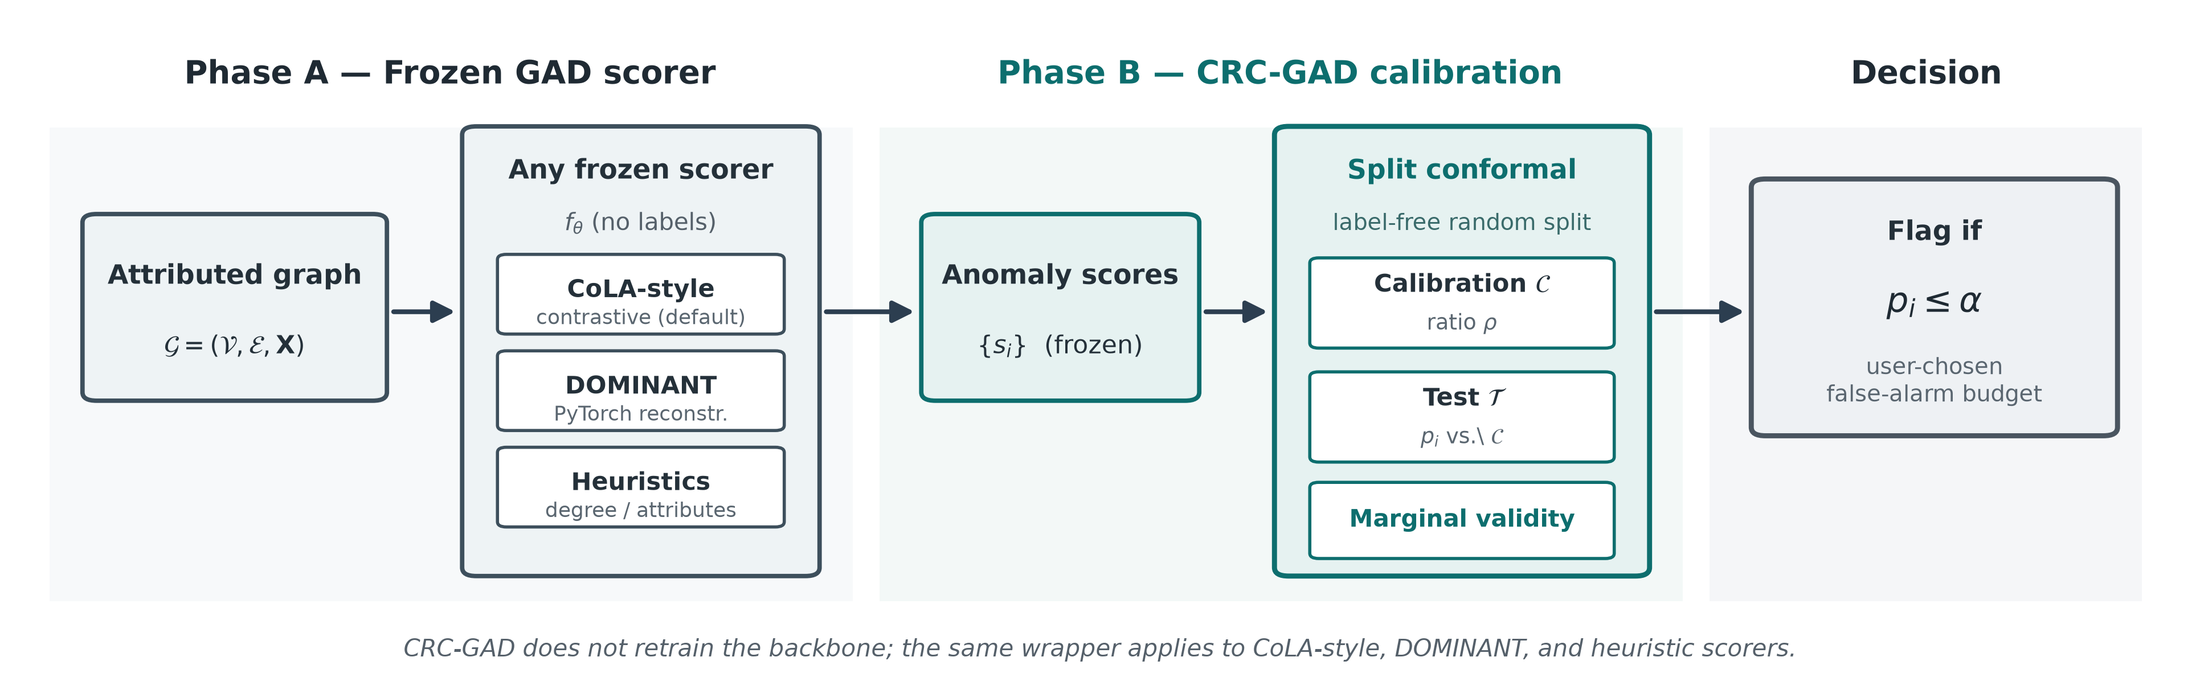
\includegraphics[width=\linewidth]{figures/pipeline.png}
\caption{Overview of CRC-GAD: a frozen score-based GAD backbone (CoLA-inspired contrastive by default; PyTorch DOMINANT and degree/attribute alternatives in experiments), split conformal calibration to $p$-values via a label-free random $\mathcal{C}/\mathcal{T}$ split, and decisions at nominal level $\alpha$. The proved guarantee is marginal random-test-node validity (Theorem~\ref{thm:randomization}).}
\label{fig:pipeline}
\end{figure*}
This design is model-agnostic: any score-based graph anomaly detector (e.g., DOMINANT, AnomalyDAE, CONAD) can serve as the backbone; the conformal layer adds marginal validity over the random calibration--test partition (Theorem~\ref{thm:randomization}), not per-node FPR guarantees.

\subsection{Graph Representation}
\label{sec:meth_preprocess}

The first stage of CRC-GAD prepares the raw attributed network for contrastive learning and conformal evaluation. We use a standard representation that is compatible with graph convolutional networks and preserves the structural and attribute information necessary for anomaly detection.

\paragraph{Feature normalization.}
The raw node attribute matrix $\mathbf{X} \in \mathbb{R}^{N \times F}$ is row-normalized so that each node's feature vector has unit $\ell_1$ norm:
\begin{equation}
\label{eq:feat_norm}
\tilde{\mathbf{x}}_i = \mathbf{x}_i / \|\mathbf{x}_i\|_1.
\end{equation}
Row normalization prevents nodes with large absolute feature magnitudes from dominating the contrastive learning objective and stabilizes training across datasets with heterogeneous feature scales. For datasets where features are already normalized (e.g., BlogCatalog, Flickr), this step is a no-op. The normalized matrix $\tilde{\mathbf{X}}$ is used as input to the GNN encoder throughout training and inference.

\paragraph{Adjacency normalization.}
The binary adjacency matrix $\mathbf{A}$ is symmetrically normalized and augmented with self-loops to form the input to the GCN encoder:
\begin{equation}
\label{eq:adj_norm}
\hat{\mathbf{A}} = \widetilde{\mathbf{D}}^{-1/2}(\mathbf{A} + \mathbf{I})\widetilde{\mathbf{D}}^{-1/2},
\end{equation}
where $\widetilde{\mathbf{D}}$ is the degree matrix of $\mathbf{A} + \mathbf{I}$. This normalization, standard in GCN-based architectures~\cite{kipf2017gcn}, prevents the scale of node representations from growing with node degree and improves gradient flow in deep layers. The self-loops ensure that every node retains a non-vanishing representation of its own features.

\paragraph{Node-set partitioning.}
To support both early stopping and conformal calibration, the node set $\mathcal{V}$ is partitioned into four disjoint subsets: $\mathcal{V}_{\text{train}}$, $\mathcal{V}_{\text{val}}$, $\mathcal{C}$, and $\mathcal{T}$ ( Eq.~\eqref{eq:partition}). The partition is constructed by uniform random shuffling {without} using score or label information.  Contrastive training uses nodes in $\mathcal{V}_{\text{train}}$ only (Section~\ref{sec:exp_implementation}); validation supports early stopping; $\mathcal{C}$ and $\mathcal{T}$ are formed from the remaining eval nodes.  Anomalies are \emph{not} excluded from $\mathcal{C}$ unless explicitly noted.

\subsection{Contrastive Learning Module}
\label{sec:meth_training}

The contrastive module is an \emph{optional default backbone} for $f_\theta$, not the contribution of CRC-GAD.  It follows the \emph{scoring principle} of~\cite{liu2022cola} (Eq.~\eqref{eq:cola_score}): multi-round positive--negative context disagreement.  \textbf{Attribution and scope:} CoLA~\cite{liu2022cola} is prior work; we do not claim it as ours.  Our pinned code (\texttt{src/crc\_gad/scorer.py}) uses a \emph{simplified CoLA-inspired} NumPy GCN scorer---two-layer message passing, neighbor-mean positive context, random negative context, and validation-AUC early stopping---rather than the full PyTorch RWR subgraph + bilinear discriminator pipeline.  Section~\ref{sec:prob_contrastive_scoring} states the CoLA reference formulation for context; primary CoLA-style numbers use the simplified scorer, while Table~\ref{tab:backbones} shows the conformal wrapper also on PyTorch DOMINANT.

\paragraph{Encoder and scoring.}
A two-layer GCN encoder maps normalized node features through $\hat{\mathbf{A}}$ (Eq.~\eqref{eq:adj_norm}).  For each node $v_i$, a positive context vector aggregates normalized neighbor embeddings; over $R$ rounds, negative contexts are drawn by permuting node embeddings.  The anomaly score averages the gap ``negative agreement minus positive agreement'' (Eq.~\eqref{eq:cola_score}, simplified).  Training updates the final layer with a lightweight contrastive signal on mini-batches from $\mathcal{V}_{\text{train}}$; checkpoint selection uses validation AUC every $E_{\text{val}}$ epochs with patience $P$ (labels used \emph{only} for early stopping, not for conformal calibration).

\subsection{Conformal Risk Control}
\label{sec:meth_conformal}

The conformal risk-control layer converts raw anomaly scores $\mathbf{s}$ into calibrated p-values satisfying $\Pr(p_i \leq \alpha) \leq \alpha$ for a uniformly random test node under the random partition (Theorem~\ref{thm:randomization}).  Expected normal-node FPR is discussed via Proposition~\ref{prop:flagged} and Section~\ref{sec:th_limitations}; we do not claim per-node conditional FPR control.

\paragraph{Calibration-test partition.}
The set of evaluation nodes $\mathcal{V}_{\text{eval}}$ (nodes not used for training or validation) is partitioned into a calibration set $\mathcal{C}$ and a test set $\mathcal{T}$ as defined in Eq.~\eqref{eq:partition}.
The partition is formed by uniform random shuffling; the calibration ratio $\rho = |\mathcal{C}| / |\mathcal{V}_{\text{eval}}|$ is a user-configurable hyperparameter (default $\rho = 0.3$). No information from scores or labels is used in the split, so under the randomness of the partition, the conformal p-value enjoys marginal validity (Theorem~\ref{thm:randomization}).

\paragraph{p-value computation and decision rule.}
For each test node $v_i \in \mathcal{T}$, the conformal p-value is computed by ranking $s_i$ among the calibration scores as in Eq.~\eqref{eq:pvalue_formal}.
A small p-value indicates that node $i$'s score is unusually large relative to the calibration population, providing evidence that $i$ is anomalous. The decision rule flags node $i$ as anomalous if $p_i \leq \alpha$ (Eq.~\eqref{eq:decision}).
Under Theorem~\ref{thm:randomization}, $\Pr(p_i \leq \alpha) \leq \alpha$ marginally over the random partition and a uniformly random test index $i \in \mathcal{T}$ (Eq.~\eqref{eq:validity}).  Expected normal-node FPR is discussed via Proposition~\ref{prop:flagged} and Section~\ref{sec:th_limitations}, not as a per-node guarantee.  Conformal AUC is computed from $\{1 - p_i\}_{i \in \mathcal{T}}$ on the test set to assess whether calibration preserves the ranking quality of the underlying scorer.

\subsection{Training Algorithm}
\label{sec:meth_algorithm}

Algorithm~\ref{alg:crcgad} summarizes the end-to-end CRC-GAD pipeline (contrastive scoring step matches our simplified implementation in Section~\ref{sec:meth_training}). The algorithm takes as input the attributed graph $\mathcal{G}$, hyperparameters (scoring rounds $R$, calibration ratio $\rho$, etc.), and the significance level $\alpha$. It outputs conformal p-values and binary decisions for all test nodes. Steps 1--2 preprocess the graph and partition the node set. Steps 3--5 train the contrastive scorer with early stopping on validation AUC. Steps 6--7 compute anomaly scores for all nodes over $R$ rounds. Steps 8--9 compute p-values and apply the decision rule for test nodes. The conformal layer is model-agnostic: any score-based graph anomaly detector can serve as the backbone~\cite{ding2019dominant,fan2020anomalydae,xu2022conad}. Table~\ref{tab:main_results} reports the pinned simplified CoLA-style scorer; Table~\ref{tab:backbones} wraps multiple alternative scorers with the same CRC-GAD layer.

\begin{algorithm}[t]
\caption{CRC-GAD pipeline.}
\label{alg:crcgad}
\begin{algorithmic}[1]
\REQUIRE Graph $\mathcal{G}=(\mathcal{V},\mathcal{E},\mathbf{X})$, significance level $\alpha \in (0,1)$, hyperparameters $(K, R, E_{\text{val}}, \texttt{max\_epochs}, \texttt{patience})$.
\ENSURE P-values $\{p_i\}_{i\in\mathcal{T}}$, decisions $\{\hat{y}_i\}_{i\in\mathcal{T}}$.
\STATE Normalize features and adjacency to obtain $\tilde{\mathbf{X}}$ (Eq.~\ref{eq:feat_norm}) and $\hat{\mathbf{A}}$ (Eq.~\ref{eq:adj_norm}).
\STATE Uniformly split nodes into $\mathcal{V}_{\text{train}}, \mathcal{V}_{\text{val}}, \mathcal{C}, \mathcal{T}$.
\STATE Initialize model parameters $\theta=\{\phi,\psi,\mathcal{R}\}$; set \texttt{best\_auc} $\gets -\infty$, \texttt{wait} $\gets 0$.
\FOR{epoch $=1$ to \texttt{max\_epochs}}
    \STATE Mini-batch contrastive update on $\mathcal{V}_{\text{train}}$ (simplified GCN scorer; Section~\ref{sec:meth_training}).
    \IF{epoch mod $E_{\text{val}} = 0$}
        \STATE Compute validation scores on $\mathcal{V}_{\text{val}}$ and AUC.
        \IF{AUC improves}
            \STATE Save checkpoint $\theta^\star$; set \texttt{wait} $\gets 0$.
        \ELSE
            \STATE \texttt{wait} $\gets$ \texttt{wait} $+ 1$.
        \ENDIF
        \IF{\texttt{wait} $\geq$ \texttt{patience}}
            \STATE \textbf{break}
        \ENDIF
    \ENDIF
\ENDFOR
\STATE Restore best checkpoint $\theta^\star$ and set evaluation mode.
\FOR{each node $i \in \mathcal{V}$}
    \STATE Compute multi-round anomaly score $s_i$ over $R$ rounds (Eq.~\ref{eq:cola_score}).
\ENDFOR
\FOR{each $i \in \mathcal{T}$}
    \STATE $p_i \gets \dfrac{1 + \#\{j \in \mathcal{C}: s_j \ge s_i\}}{1 + |\mathcal{C}|}$ \hfill (Eq.~\ref{eq:pvalue_formal})
    \STATE $\hat{y}_i \gets \mathbb{1}[p_i \le \alpha]$ \hfill (Eq.~\ref{eq:decision})
\ENDFOR
\RETURN $\{p_i, \hat{y}_i\}_{i\in\mathcal{T}}$.
\end{algorithmic}
\end{algorithm}

\subsection{Complexity Analysis}
\label{sec:meth_complexity}

We analyze the computational cost of each stage of CRC-GAD. 

\textbf{Preprocessing:} Feature normalization is $O(N \cdot F)$; adjacency normalization is $O(N + |\mathcal{E}|)$. \textbf{Training:} Each epoch runs mini-batch contrastive updates on the simplified GCN scorer; cost scales as $O(T \cdot B \cdot L \cdot d)$ for $T$ epochs, batch size $B$, $L$ layers, embedding $d$. \textbf{Scoring:} Computing $\mathbf{s}$ over $R$ rounds costs $O(R \cdot N \cdot d)$ in our implementation. \textbf{Conformal calibration:} For each test node, a linear scan over $\mathcal{C}$ yields $O(|\mathcal{T}| \cdot |\mathcal{C}|)$; in practice this is under one second for our benchmarks. The conformal layer adds negligible overhead compared to training and multi-round scoring.

\subsection{Theoretical Analysis}
\label{sec:theory}

This subsection provides the formal theoretical foundations underpinning CRC-GAD, immediately following the algorithmic description so that methodological and analytical content appear in one place. We present the core marginal validity guarantee under random partition (Section~\ref{sec:th_validity}), analyze what happens when scores contain ties (Section~\ref{sec:th_ties}), state the randomization-based validity and its relation to exchangeability (Section~\ref{sec:th_exchangeability}), discuss empirical stability of the FPR (Section~\ref{sec:th_finitesample}), and prove that conformal calibration preserves the ranking quality of the underlying scorer (Section~\ref{sec:th_ranking}).  We conclude with assumptions and limitations (Section~\ref{sec:th_limitations}).
\subsubsection{Marginal Validity of Conformal p-values}
\label{sec:th_validity}

We state the central guarantee in two equivalent forms: first under exchangeability (standard in the conformal literature), then under the randomization scheme used in CRC-GAD.  Let $\mathcal{C} = \{v_1, \ldots, v_n\}$ be the calibration set and $v_{n+1} \in \mathcal{T}$ a test node.  Let $s_1, \ldots, s_n, s_{n+1}$ denote their respective anomaly scores, produced by a fixed (frozen) scoring model.

\begin{definition}[Exchangeability]
\label{def:exchangeable}
A finite sequence of random variables $Z_1, \ldots, Z_{n+1}$ is {exchangeable} if, for every permutation $\pi$ of $\{1, \ldots, n+1\}$,
\begin{equation}
\label{eq:exchangeable}
    (Z_1, \ldots, Z_{n+1}) \;\overset{d}{=}\; (Z_{\pi(1)}, \ldots, Z_{\pi(n+1)}).
\end{equation}
That is, the joint distribution is invariant under reordering.  Note that i.i.d.\ random variables are exchangeable, but exchangeability is strictly weaker than independence.
\end{definition}

\begin{theorem}[Marginal validity under exchangeability]
\label{thm:marginal_full}
Suppose the scores $s_1, \ldots, s_n, s_{n+1}$ are exchangeable.  Define the conformal p-value of the test node as
\begin{equation}
\label{eq:pval_thm}
    p_{n+1} = \frac{1 + \sum_{j=1}^{n}\mathbb{1}[s_j \geq s_{n+1}]}{1 + n}.
\end{equation}
Then, for any $\alpha \in [0, 1]$,
\begin{equation}
\label{eq:validity_thm}
    \Pr(p_{n+1} \leq \alpha) \;\leq\; \alpha.
\end{equation}
\end{theorem}

\begin{proof}
Define the {rank} of the test score among all $n + 1$ scores:
\begin{equation}
\label{eq:rank}
    R_{n+1} = 1 + \sum_{j=1}^{n}\mathbb{1}[s_j \geq s_{n+1}].
\end{equation}
The p-value is then $p_{n+1} = R_{n+1}/(n + 1)$.  By exchangeability, the joint distribution of $(s_1, \ldots, s_{n+1})$ is invariant under permutations.  Consequently, the rank of any individual element is uniformly distributed over $\{1, 2, \ldots, n+1\}$ in the following sense:
\begin{equation}
\label{eq:uniform_rank}
    \Pr(R_{n+1} = k) \;=\; \frac{1}{n+1}, \qquad k = 1, \ldots, n+1,
\end{equation}
when the scores are almost surely distinct (we address ties in Section~\ref{sec:th_ties}).

Now, the event $\{p_{n+1} \leq \alpha\}$ is equivalent to $\{R_{n+1} \leq \alpha(n+1)\}$, which is equivalent to $\{R_{n+1} \leq \lfloor \alpha(n+1) \rfloor\}$ since $R_{n+1}$ is an integer.  Therefore:
\begin{multline}
\label{eq:prob_bound}
    \Pr(p_{n+1} \leq \alpha)
    = \Pr\bigl(R_{n+1} \leq \lfloor\alpha(n+1)\rfloor\bigr)\\
    = \frac{\lfloor\alpha(n+1)\rfloor}{n+1} \;\leq\; \alpha.
\end{multline}
The inequality follows from the elementary fact that $\lfloor x \rfloor \leq x$ for all $x \in \mathbb{R}$.
\end{proof}

\begin{theorem}[Marginal validity under randomization (CRC-GAD)]
\label{thm:randomization}
Let $\theta^*$ denote the trained model parameters and let $\mathbf{s} = (s_i)_{i \in \mathcal{V}_{\text{eval}}}$ be the score vector computed by $f_{\theta^*}$.  Suppose $(\mathcal{C}, \mathcal{T})$ is a uniformly random partition of $\mathcal{V}_{\text{eval}}$ with $|\mathcal{C}| = n$.  For a test node $v_i$ chosen uniformly at random from $\mathcal{T}$, the conformal p-value $p_i$ in Eq.~\eqref{eq:pvalue_formal} satisfies $\Pr(p_i \leq \alpha) \leq \alpha$ for all $\alpha \in [0,1]$, where the probability is over the random partition and the random choice of test node.
\end{theorem}

\begin{proof}
Fix the trained model parameters $\theta^*$ and the resulting score vector $\mathbf{s} = (s_i)_{i \in \mathcal{V}_{\text{eval}}}$.  The scores are deterministic conditional on $\theta^*$.  The partition $(\mathcal{C}, \mathcal{T})$ is chosen uniformly at random among all $\binom{|\mathcal{V}_{\text{eval}}|}{n}$ splits of $\mathcal{V}_{\text{eval}}$, and the test node $v_i$ is chosen uniformly at random from $\mathcal{T}$.  The combined experiment of (i)~choosing the partition and (ii)~selecting the test node is equivalent to selecting a uniformly random ordered pair (test index, remaining set) from $\mathcal{V}_{\text{eval}}$.  Conditional on $\mathbf{s}$, each node in $\mathcal{V}_{\text{eval}}$ is equally likely to occupy the test role.  Therefore the rank of $s_i$ among the $n+1$ scores $\{s_j\}_{j \in \mathcal{C}} \cup \{s_i\}$ is uniformly distributed over $\{1, \ldots, n+1\}$ by symmetry of the uniform random selection.  Applying the argument of Theorem~\ref{thm:marginal_full} verbatim gives $\Pr(p_i \leq \alpha) \leq \alpha$.
\end{proof}

\begin{remark}
Theorem~\ref{thm:randomization} is the operative guarantee in CRC-GAD.  Unlike Theorem~\ref{thm:marginal_full}, it does not require node scores to be exchangeable or independent; validity follows solely from the randomness of the partition.  Section~\ref{sec:th_exchangeability} further discusses how this randomization-based validity relates to the standard exchangeability assumption in conformal prediction.
\end{remark}

\begin{remark}
The guarantee in Theorem~\ref{thm:marginal_full} is {marginal}: it holds for each test node individually, averaging over the randomness in the calibration--test partition and any stochasticity in the scoring process.  It does not require the scores to have any particular distributional form (Gaussian, exponential, etc.)-it is entirely {distribution-free}.  Furthermore, it holds in {finite samples}: there is no need for $n \to \infty$ asymptotics.  These properties make conformal p-values uniquely suited to the graph anomaly detection setting, where score distributions are complex, dataset sizes vary widely, and practitioners need guarantees that hold for the specific dataset at hand.
\end{remark}

\subsubsection{Handling Ties}
\label{sec:th_ties}

The proof above assumes almost surely distinct scores.  When ties are present-i.e., when $\Pr(s_i = s_j) > 0$ for some $i \neq j$-the rank $R_{n+1}$ is no longer uniformly distributed.  However, the validity guarantee still holds, and in fact becomes {conservative} (the p-value is stochastically larger than uniform).
\begin{proposition}[Validity under ties]
\label{prop:ties}
If $s_1, \ldots, s_{n+1}$ are exchangeable (possibly with ties), then the conformal p-value in Eq.~\eqref{eq:pval_thm} satisfies $\Pr(p_{n+1} \leq \alpha) \leq \alpha$ for all $\alpha \in [0,1]$.
\end{proposition}
\begin{proof}
The $+1$ in the numerator of $p_{n+1}$ ensures that $R_{n+1} \geq 1$ always, so $p_{n+1} \geq 1/(n+1) > 0$.  When ties occur, the count $\sum_{j=1}^{n}\mathbb{1}[s_j \geq s_{n+1}]$ includes all calibration scores tied with $s_{n+1}$, which {inflates} $R_{n+1}$ and hence $p_{n+1}$.  Formally, for any fixed realization of the score values (ignoring which score is assigned to which index), exchangeability implies that each of the tied scores is equally likely to be the test score, and the $+1$ in the numerator ensures the p-value is never below $1/(n+1)$ even in the worst case.  A detailed proof by coupling with a tie-breaking randomization is given in~\cite{vovk2005algorithmic}, Chapter 8.
\end{proof}
In practice, the raw scores are continuous-valued (real-valued outputs of a neural network followed by sigmoid and averaging), so exact ties are astronomically unlikely.  Our experiments report empirical FPR near nominal $\alpha$ on Cora/Citeseer/PubMed where the scorer attains reasonable AUC; when the backbone ranks below chance (BlogCatalog, Flickr), detection power collapses and FPR control can become anti-conservative (Table~\ref{tab:main_results}), consistent with Section~\ref{sec:th_limitations}.

\subsubsection{Exchangeability and the Random Partition}
\label{sec:th_exchangeability}

The standard conformal guarantee (Theorem~\ref{thm:marginal_full}) is stated under exchangeability of the scores.  On graphs, nodes are typically {not} independent: neighboring nodes share edges and, after GNN message passing, their representations (and hence scores) can be dependent.  We do {not} claim that a random node split automatically makes scores exchangeable; graph structure can induce dependencies that persist regardless of the partition. Instead, CRC-GAD relies on {randomization validity}: the calibration set $\mathcal{C}$ is a uniformly random subset of $\mathcal{V}_{\text{eval}}$, and the test node is drawn uniformly from $\mathcal{T} = \mathcal{V}_{\text{eval}} \setminus \mathcal{C}$.  The scores are computed by a {fixed} model $f_\theta$ on the {fixed} graph; the only randomness is in the partition.  Under this randomization, the conformal p-value satisfies $\Pr(p_i \leq \alpha) \leq \alpha$ {marginally} over the random partition and the random choice of test node.  No assumption on the joint distribution of node scores (exchangeability or independence) is required; the guarantee holds by symmetry of the random split.

The validity guarantee under random partition follows directly from Theorem~\ref{thm:randomization} (Section~\ref{sec:th_validity}), which establishes $\Pr(p_i \leq \alpha) \leq \alpha$ by the symmetry of the uniform random partition, without requiring exchangeability or independence of node scores.

\paragraph{When might validity be violated?}
Validity can be compromised if (i)~the partition depends on the scores or labels (e.g., placing high-scoring nodes in $\mathcal{T}$); (ii)~the model is retrained or fine-tuned using the calibration set; or (iii)~the calibration set is heavily contaminated with anomalies, so that the ``reference'' distribution no longer reflects normal nodes.  CRC-GAD avoids (i) and (ii) by using a score-agnostic uniform shuffle and a frozen model.  For (iii), we provide an extended discussion in Section~\ref{sec:th_limitations} and a controlled stress test in Section~\ref{sec:abl_contamination}.
\subsubsection{Empirical FPR and Stability}
\label{sec:th_finitesample}

Theorem~\ref{thm:marginal_full} provides a bound on the {marginal} probability $\Pr(p_i \leq \alpha)$ for a single test node.  In practice, we observe the {empirical} FPR over all normal test nodes:
\begin{equation}
\label{eq:empirical_fpr}
    \widehat{\text{FPR}}(\alpha) = \frac{1}{|\mathcal{T}_0|}\sum_{i \in \mathcal{T}_0}\mathbb{1}[p_i \leq \alpha],
\end{equation}
where $\mathcal{T}_0 = \{i \in \mathcal{T} : y_i = 0\}$ is the set of normal test nodes.  By marginal random-test-node validity (Theorem~\ref{thm:randomization}), $\Pr(p_i\leq\alpha)\leq\alpha$ for a uniformly random test index; this does \emph{not} by itself imply $\mathbb{E}[\widehat{\text{FPR}}(\alpha)]\leq\alpha$ without the normal-node bridge in Section~\ref{sec:th_limitations}. The empirical FPR across test nodes is not independent (test nodes share the same calibration set $\mathcal{C}$), so standard concentration inequalities that assume independence (e.g., Hoeffding) do not apply without further assumptions. We therefore do not state a formal concentration bound; instead, we report mean $\pm$ standard deviation over seeds $\{0,1,2,3,4\}$ (and multi-dataset studies where noted) as empirical uncertainty intervals. Table~\ref{tab:abl_alpha} and Table~\ref{tab:main_results} report observed FPR/flagged rates; identity gaps in the CSV are $\approx 0$ (Proposition~\ref{prop:flagged}).

\subsubsection{Preservation of Ranking Quality}
\label{sec:th_ranking}

A natural concern is whether conformal calibration degrades the discriminative performance of the underlying anomaly scores.  We show that, under mild conditions, the conformal transformation exactly preserves the ranking.

\begin{proposition}[Rank preservation]
\label{prop:rank}
Let $s_i$ and $s_j$ be the anomaly scores of two test nodes $v_i, v_j \in \mathcal{T}$, computed by the same frozen model, and let $p_i$ and $p_j$ be their conformal p-values computed against the same calibration set $\mathcal{C}$.  If $s_i > s_j$, then $p_i \leq p_j$ (equivalently, $1 - p_i \geq 1 - p_j$).
\end{proposition}

\begin{proof}
By definition,
\begin{equation}
    p_i = \frac{1 + \sum_{k \in \mathcal{C}}\mathbb{1}[s_k \geq s_i]}{1 + |\mathcal{C}|}, \qquad
    p_j = \frac{1 + \sum_{k \in \mathcal{C}}\mathbb{1}[s_k \geq s_j]}{1 + |\mathcal{C}|}.
\end{equation}
Since $s_i > s_j$, for every $k \in \mathcal{C}$, $\mathbb{1}[s_k \geq s_i] \leq \mathbb{1}[s_k \geq s_j]$ (if $s_k$ is at least as large as $s_i$, it is certainly at least as large as $s_j$, but not conversely).  Summing over $k$:
\begin{equation}
    \sum_{k \in \mathcal{C}}\mathbb{1}[s_k \geq s_i] \;\leq\; \sum_{k \in \mathcal{C}}\mathbb{1}[s_k \geq s_j],
\end{equation}
which implies $p_i \leq p_j$.
\end{proof}

\begin{corollary}[AUC preservation]
\label{cor:auc}
When both AUCs are computed on the same node set $\mathcal{T}$ with no ties, the conformal AUC equals the raw AUC on $\mathcal{T}$.  In practice, small differences may arise because: (i)~the raw AUC is computed on all nodes while the conformal AUC is computed only on $\mathcal{T}$; and (ii)~rare ties among continuous raw scores can affect ordering.  Under these practical conditions, the conformal scores $\{1 - p_i\}_{i \in \mathcal{T}}$ induce the same pairwise ordering over test nodes as the raw scores $\{s_i\}_{i \in \mathcal{T}}$.  Consequently,
\begin{multline}
    \mathrm{AUC}_{\mathrm{conformal}} = \mathrm{AUC}\!\left(\{y_i\}_{i \in \mathcal{T}},\, \{1 - p_i\}_{i \in \mathcal{T}}\right) \\
    = \mathrm{AUC}\!\left(\{y_i\}_{i \in \mathcal{T}},\, \{s_i\}_{i \in \mathcal{T}}\right)
\end{multline}
\end{corollary}

\begin{proof}
AUC depends only on the pairwise ordering of scores between positive (anomalous) and negative (normal) examples.  By Proposition~\ref{prop:rank}, $1 - p_i > 1 - p_j$ if and only if $s_i > s_j$.  Since both scoring schemes induce identical orderings, the AUC is identical.
\end{proof}

\subsubsection{Assumptions and limitations}
\label{sec:th_limitations}

\paragraph{Graph dependence.}
Graph structure induces dependencies between node scores.  The marginal validity guarantee holds under the {random partition} only; expected normal-node FPR is at most $\alpha$ under the bridge in Remark after Proposition~\ref{prop:flagged}, not for every individual node.

\paragraph{Calibration set contamination.}
Split conformal validity for normal nodes assumes that calibration scores approximate the null (normal) reference law.  If a fraction $\pi_{\mathcal{C}}$ of calibration nodes are anomalous, the empirical calibration distribution is a mixture of normal and anomaly score laws.  Let $S^{(0)}$ and $S^{(1)}$ denote scores for normal and anomalous nodes.  For a normal test score $s \sim S^{(0)}$, the conformal rank statistic in Eq.~\eqref{eq:pvalue_formal} compares $s$ against a calibration sample drawn from $(1-\pi_{\mathcal{C}})S^{(0)} + \pi_{\mathcal{C}} S^{(1)}$.  When anomalies receive \emph{higher} scores than most normals (the usual case in our benchmarks), high-scoring anomalies in $\mathcal{C}$ inflate the rank counts for normal test nodes, yielding \emph{larger} p-values and a \emph{conservative} empirical FPR (below $\alpha$).  Conversely, if camouflaged anomalies receive scores comparable to or below typical normals, contamination can \emph{deflate} ranks and produce \emph{anti-conservative} FPR inflation---the failure mode most relevant operationally when the calibration pool is not curated.  The guarantee in Theorem~\ref{thm:randomization} is stated for a clean calibration reference; contamination breaks the idealized exchangeability/mixture interpretation without necessarily destroying ranking quality (Proposition~\ref{prop:rank}).
In our evaluation protocol (Section~\ref{sec:exp_injection}), the global anomaly rate is 5\%.  Section~\ref{sec:abl_contamination} increases $\pi_{\mathcal{C}}$ by moving anomalies from $\mathcal{T}$ into $\mathcal{C}$: empirical FPR among normals \emph{decreases} (conservative), consistent with theory.
\paragraph{Marginal vs.\ conditional guarantees.}
Theorem~\ref{thm:randomization} controls the FPR \emph{marginally} over the random calibration--test partition.  It does not promise node-wise conditional error control for every subgraph or degree group: graph dependence (previous paragraph) and covariate shift across communities can make local FPR differ from $\alpha$ even when the global empirical FPR tracks $\alpha$ (Section~\ref{sec:th_finitesample}).  Reporting stratified FPR by degree quantile is a useful diagnostic; we report it on Cora in Section~\ref{sec:abl_degree}.
\paragraph{Operational scope.}
CRC-GAD controls false positives among \emph{normal} test nodes; it does not bound false negatives or provide anomaly-level coverage.  The conformal layer adds $O(n)$ ranking cost after scoring and does not remove the need for a strong unsupervised scorer on highly imbalanced or evolving graphs.  These scope limits are intentional: the framework targets deployments where an explicit false-alarm budget matters~\cite{bates2023testing,ma2021comprehensive}.
\paragraph{Summary.}
Section~\ref{sec:abl_contamination} empirically complements the contamination discussion above.
The theoretical analysis establishes four key properties of CRC-GAD: (1)~marginal validity at any significance level $\alpha$ (Theorem~\ref{thm:marginal_full}), including under ties (Proposition~\ref{prop:ties}); (2)~validity under the random partition without assuming node independence (Theorem~\ref{thm:randomization}); (3)~empirical reporting of FPR/flagged rate across seeds and datasets (Section~\ref{sec:th_finitesample}); and (4)~exact preservation of the ranking quality of the underlying scorer on a fixed test set (Proposition~\ref{prop:rank} and Corollary~\ref{cor:auc}).  Together, these results show that CRC-GAD adds explicit finite-sample p-value semantics to score-based graph anomaly detectors without changing their pairwise ordering on $\mathcal{T}$.

\section{Experiments}
\label{sec:experiments}

Having presented the unified methodology and theoretical analysis in Section~\ref{sec:method}, we now evaluate CRC-GAD empirically. This section assesses CRC-GAD on public attributed-network benchmarks.
We describe datasets and anomaly injection (Section~\ref{sec:exp_datasets}--\ref{sec:exp_injection}), baselines (Section~\ref{sec:exp_baselines}), metrics (Section~\ref{sec:exp_metrics}), implementation (Section~\ref{sec:exp_implementation}), and ablations (Section~\ref{sec:ablations}).


\subsection{Datasets}
\label{sec:exp_datasets}

We evaluate CRC-GAD on six injected benchmark attributed networks: Cora, Citeseer, PubMed, ACM, BlogCatalog, and Flickr.  Table~\ref{tab:datasets} summarizes statistics.  Node features and anomaly injection follow~\cite{ding2019dominant,liu2022cola}.  ACM and Flickr load from \texttt{data/*.mat} (see \texttt{scripts/download\_datasets.py}); BlogCatalog requires the same \texttt{.mat} file---download manually if the mirror is unreachable.  As an organic proxy (not fraud labels), Section~\ref{sec:abl_organic} treats the rarest Planetoid class on Cora as the anomaly class.  Large-scale (ogbn-arxiv) and true organic-label (YelpChi) benchmarks remain future work under the same pinned protocol.

\subsection{Anomaly Injection}
\label{sec:exp_injection}

Following~\cite{ding2019dominant,liu2022cola}, we inject structural (dense cliques) and attribute anomalies via \texttt{src/crc\_gad/inject\_anomaly.py}.  Anomaly rate is 5\% by default; anomalies remain in both $\mathcal{C}$ and $\mathcal{T}$ (label-free split).

\subsection{Baseline Methods}
\label{sec:exp_baselines}

Table~\ref{tab:main_results} reports \emph{our re-runs only} under a shared injected-anomaly protocol (seeds $\{0,\ldots,4\}$); we do not copy literature AUC values.  Row ``CoLA backbone'' is raw AUC from the frozen \emph{simplified} contrastive scorer (Section~\ref{sec:meth_training}); ``CRC-GAD'' adds conformal AUC and calibration metrics at $\alpha=0.05$, including flagged rate (Proposition~\ref{prop:flagged}).  Table~\ref{tab:backbones} wraps the same CRC-GAD layer around a \emph{PyTorch DOMINANT} reimplementation matching Ding et al.'s architecture~\cite{ding2019dominant}, a lighter NumPy DOMINANT-style scorer, and degree/attribute heuristics. Full CONAD re-runs under identical injection remain complementary future work.

\textbf{Reading the table.} Empirical FPR tracks $\alpha{=}0.05$ on Cora, Citeseer, PubMed, and Flickr, but exceeds $\alpha$ on ACM ($0.051$) and BlogCatalog ($0.055$).  Backbone AUC is strong on Planetoid graphs yet \emph{below chance} on BlogCatalog ($0.365$) and Flickr ($0.342$): the simplified scorer inverts the ranking there, so TPR collapses below the flagged rate.  This is exactly the failure mode predicted in Section~\ref{sec:th_limitations} when anomalous scores do not dominate normal scores.  The ``Theory expected flagged'' row is the finite-sample bound $\lfloor\alpha(n{+}1)\rfloor/(n{+}1)$ on the \emph{expected} mixed flagged rate; observed rates may sit slightly above it on a finite number of seeds because the theorem is an expectation, not a per-split hard cap.  Across all 30 runs and four $\alpha$ levels, the flagged-rate identity gap is at most $2.8\times 10^{-17}$ (machine zero), confirming internal consistency of every reported FPR/TPR/flagged triple.

\begin{table*}[pos=t]
\centering
\caption{Reproduced results (mean $\pm$ std, 5 seeds) on six datasets from \texttt{results/main\_results.csv}. ``Theory expected flagged'' is $\lfloor\alpha(n{+}1)\rfloor/(n{+}1)$; observed flagged rates are seed means and may exceed it slightly. Max identity gap is the largest absolute violation of Proposition~\ref{prop:flagged} across seeds and $\alpha\in\{0.01,0.02,0.05,0.10\}$.}
\label{tab:main_results}
\resizebox{\linewidth}{!}{%
\begin{tabular}{lcccccc}
\toprule
\textbf{Metric} & Cora & Citeseer & Pubmed & Acm & Blogcatalog & Flickr \\
\midrule
CoLA backbone AUC (raw) & 0.776$\pm$0.009 & 0.808$\pm$0.011 & 0.592$\pm$0.014 & 0.668$\pm$0.033 & 0.365$\pm$0.015 & 0.342$\pm$0.012 \\
CRC-GAD conformal AUC & 0.768$\pm$0.076 & 0.789$\pm$0.030 & 0.576$\pm$0.022 & 0.675$\pm$0.045 & 0.357$\pm$0.020 & 0.342$\pm$0.010 \\
FPR @ $\alpha{=}0.05$ & 0.040$\pm$0.012 & 0.024$\pm$0.010 & 0.029$\pm$0.003 & 0.051$\pm$0.008 & 0.055$\pm$0.005 & 0.045$\pm$0.014 \\
TPR @ $\alpha{=}0.05$ & 0.380$\pm$0.197 & 0.471$\pm$0.081 & 0.492$\pm$0.013 & 0.113$\pm$0.065 & 0.036$\pm$0.014 & 0.043$\pm$0.014 \\
Flagged rate @ $0.05$ & 0.056$\pm$0.020 & 0.044$\pm$0.012 & 0.053$\pm$0.003 & 0.054$\pm$0.010 & 0.054$\pm$0.005 & 0.045$\pm$0.013 \\
Theory max flagged @ $0.05$ & 0.048$\pm$0.000 & 0.050$\pm$0.000 & 0.050$\pm$0.000 & 0.050$\pm$0.000 & 0.050$\pm$0.000 & 0.049$\pm$0.000 \\
\bottomrule
\end{tabular}
}

\end{table*}


\begin{figure}[pos=t]
\centering
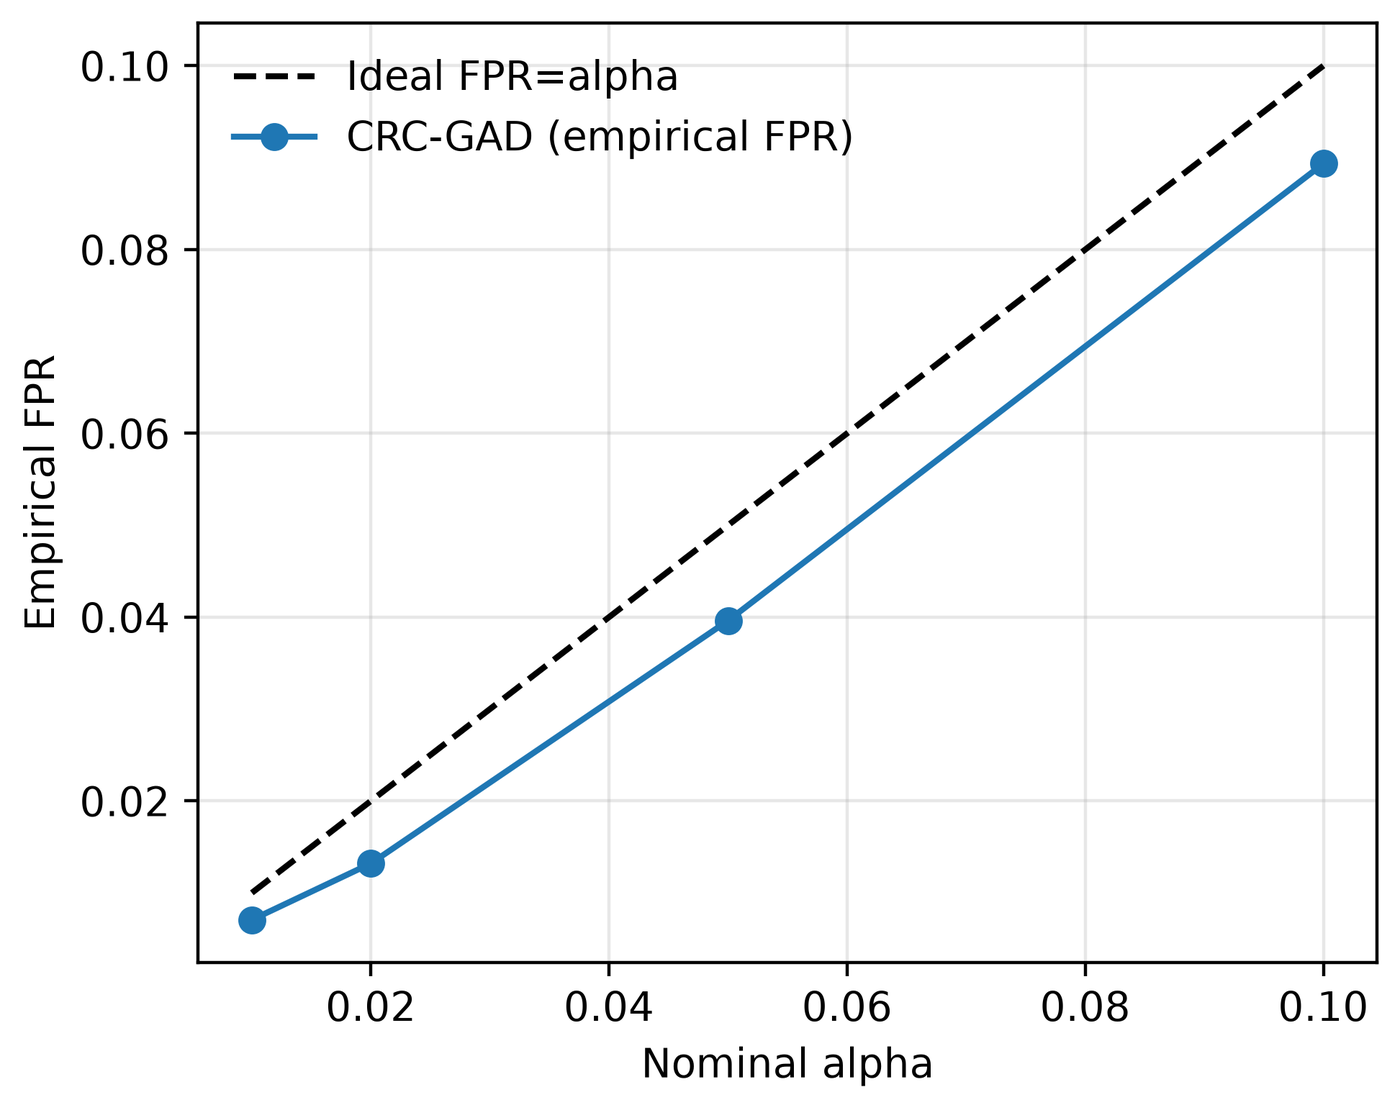
\includegraphics[width=0.9\linewidth]{figures/fig2_fpr_control.png}
\caption{Empirical FPR versus nominal $\alpha$ on Cora (from \texttt{results/main\_results.csv}); dashed line is $\mathrm{FPR}=\alpha$. See Table~\ref{tab:abl_alpha} and Table~\ref{tab:exp_conformal_compare}.}
\label{fig:fpr_control}
\end{figure}

\begin{figure}[pos=t]
\centering
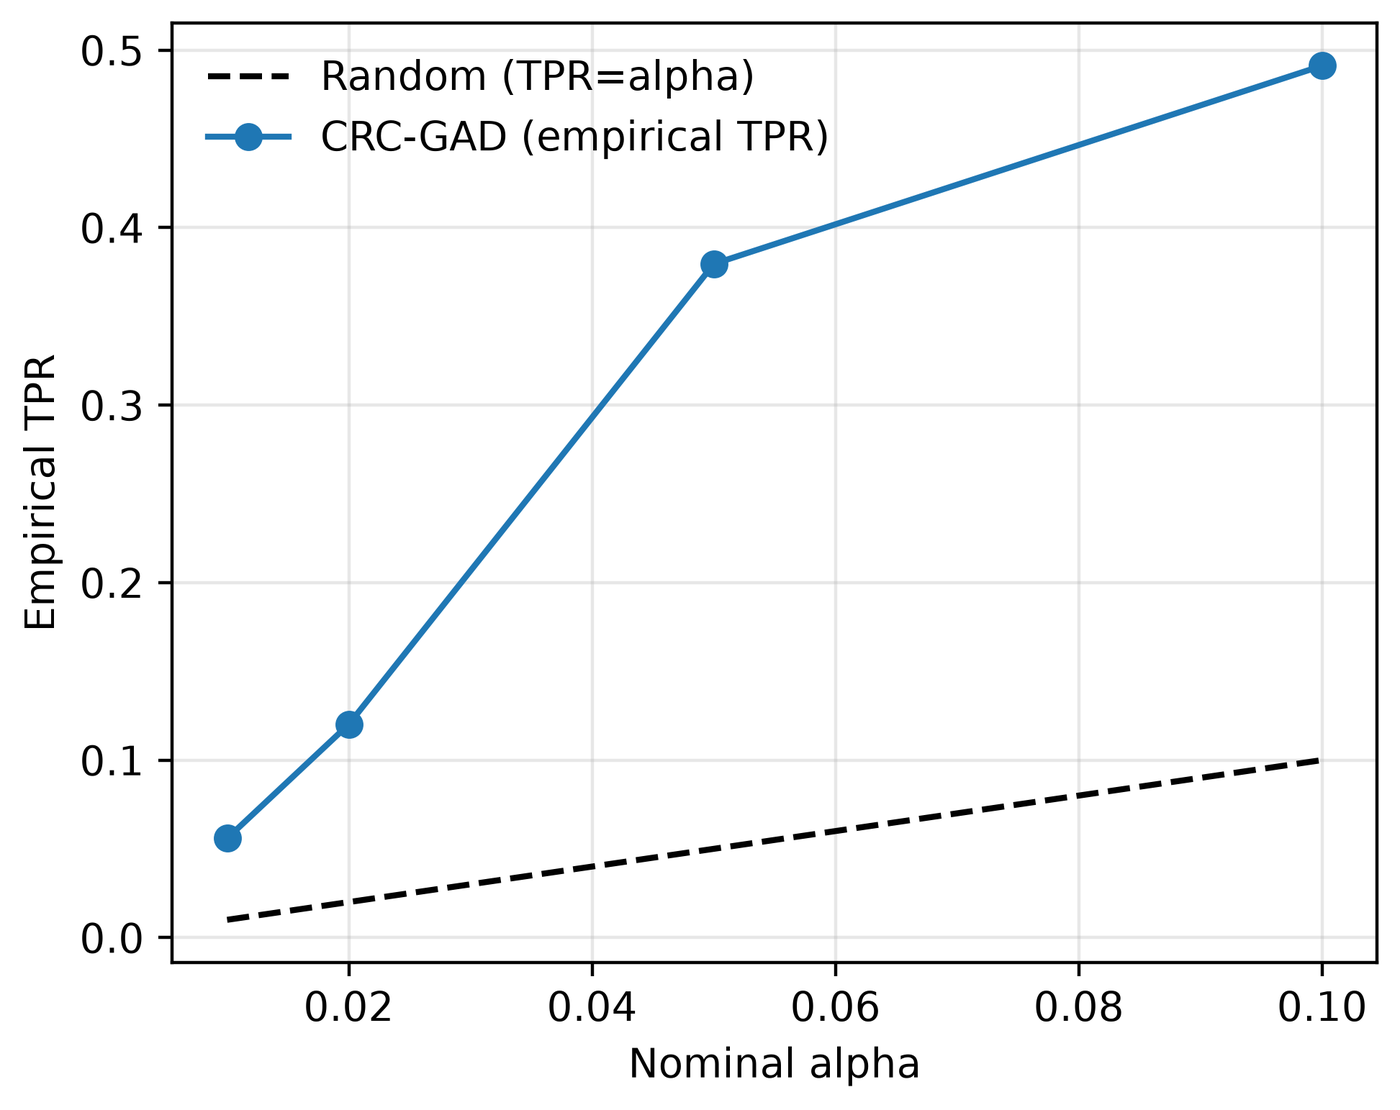
\includegraphics[width=0.9\linewidth]{figures/fig3_tpr_power.png}
\caption{Empirical TPR versus nominal $\alpha$ on Cora (from CSV). TPR is not guaranteed; it depends on backbone AUC.}
\label{fig:tpr_power}
\end{figure}

\begin{figure}[pos=t]
\centering
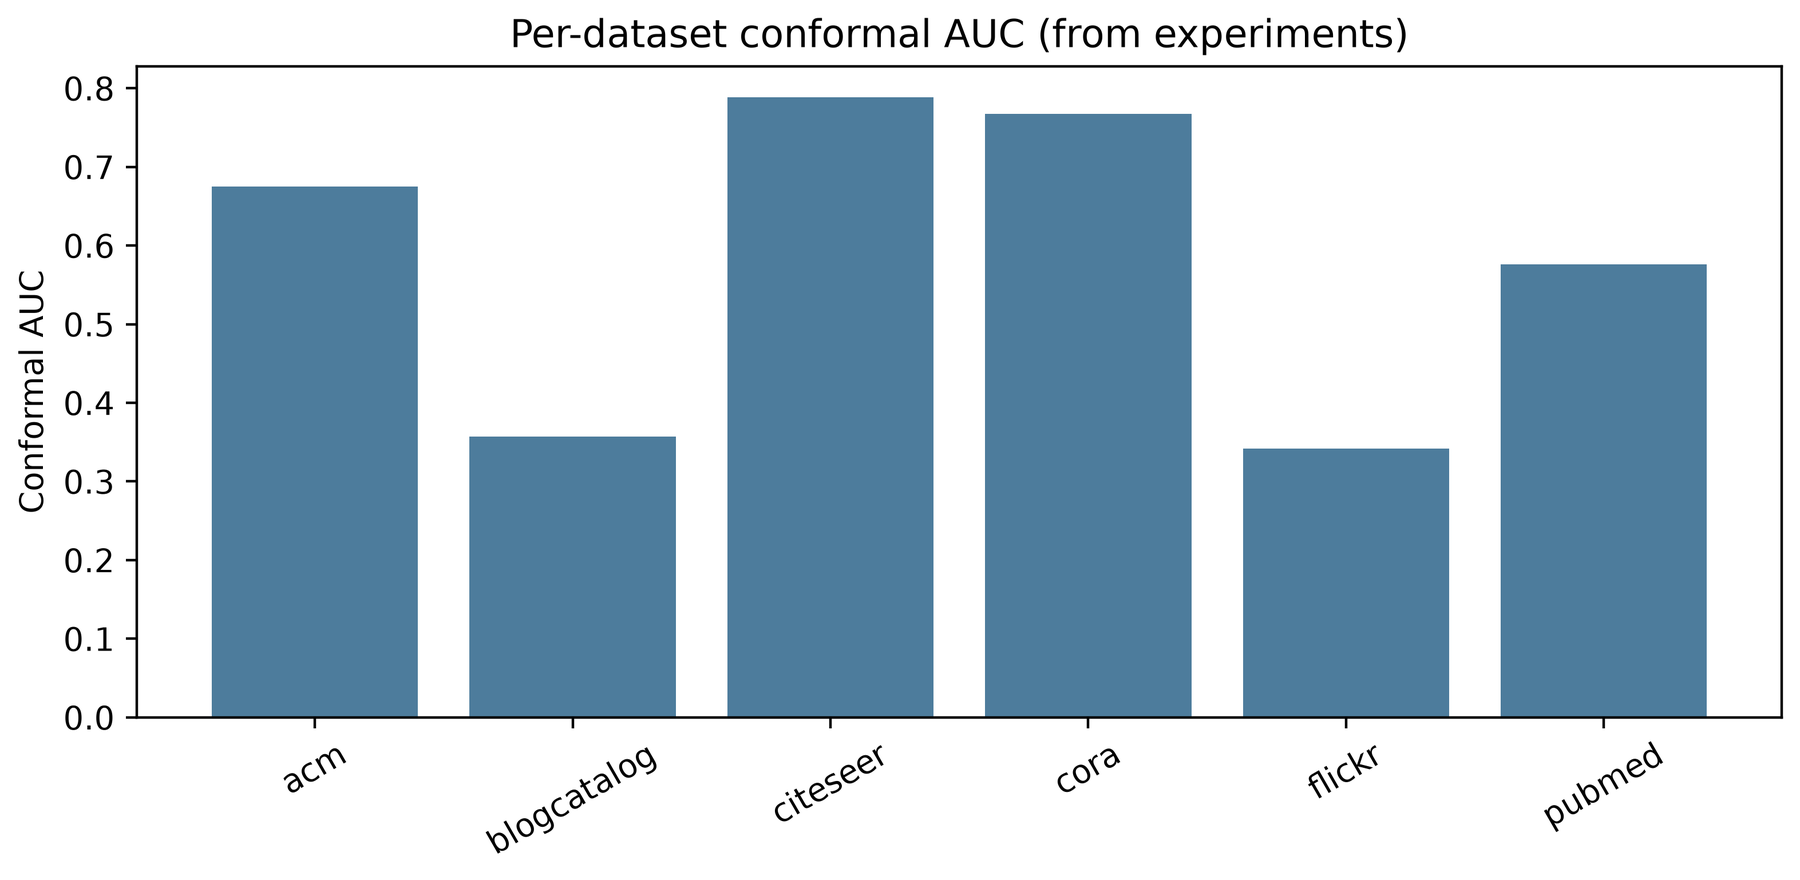
\includegraphics[width=\linewidth]{figures/fig4_per_dataset_fpr_tpr.png}
\caption{Per-dataset conformal AUC from \texttt{results/main\_summary.json} (Table~\ref{tab:main_results}).}
\label{fig:per_dataset_fpr_tpr}
\end{figure}


\subsection{Evaluation Metrics}
\label{sec:exp_metrics}

To comprehensively assess CRC-GAD, we evaluate both discriminative performance and calibration quality:
\begin{itemize}
    \item \textbf{Raw AUC:} the area under the ROC curve computed from the raw anomaly scores $\mathbf{s}$ on all nodes; it measures the discriminative power of the underlying scorer.
    \item \textbf{Conformal AUC:} the area under the ROC curve computed from the conformal scores $1 - p_i$ on the test set $\mathcal{T}$; it measures whether calibration preserves or degrades the ranking.
    \item \textbf{Empirical FPR and TPR at level $\alpha$:}
    \begin{equation}
    \label{eq:fpr_tpr}
    \begin{aligned}
    \widehat{\mathrm{FPR}}(\alpha) &= 
    \frac{\sum_{i \in \mathcal{T}} \mathbb{1}[p_i \leq \alpha] \cdot \mathbb{1}[y_i = 0]}
    {\sum_{i \in \mathcal{T}} \mathbb{1}[y_i = 0]}, \\[4pt]
    \widehat{\mathrm{TPR}}(\alpha) &= 
    \frac{\sum_{i \in \mathcal{T}} \mathbb{1}[p_i \leq \alpha] \cdot \mathbb{1}[y_i = 1]}
    {\sum_{i \in \mathcal{T}} \mathbb{1}[y_i = 1]}.
    \end{aligned}
    \end{equation}
\end{itemize}
By Theorem~\ref{thm:randomization}, marginal validity $\Pr(p_i \leq \alpha) \leq \alpha$ holds for a uniformly random test node over the random partition; the bridge to $\widehat{\mathrm{FPR}}(\alpha)$ on normal nodes is in Section~\ref{sec:th_limitations}. The empirical TPR (detection power) is not guaranteed but depends on backbone AUC (Table~\ref{tab:main_results}). We report empirical FPR and TPR at $\alpha \in \{0.01, 0.02, 0.05, 0.10\}$, the FPR gap $|\widehat{\mathrm{FPR}}(\alpha) - \alpha|$, and the flagged rate (fraction of test nodes with $p_i \leq \alpha$).


\subsection{Implementation Details}
\label{sec:exp_implementation}

Experiments use Python~3.13, NumPy/SciPy, and scikit-learn (\texttt{requirements.txt}).
\textbf{Protocol:} train 60\%, val 10\% of remainder, eval split into $\mathcal{C}$ ($\rho=0.3$) and $\mathcal{T}$ (label-free; \texttt{docs/CALIBRATION\_SET\_AUDIT.md}).
\textbf{Defaults} (\texttt{src/crc\_gad/config.py}): $d{=}128$, $K{=}8$, $M{=}5$, $R{=}32$, $\rho{=}0.3$, Adam lr $0.001$, max 120 epochs, val every 10 epochs, patience 10.
\textbf{Reproduce:} \texttt{scripts/run\_experiments.py} $\to$ \texttt{results/main\_results.csv}; tables via \texttt{scripts/generate\_paper\_tables.py}.
Code: \url{https://github.com/Amaanullakhan/CRC_GAD} (tag \texttt{v1.0-rebuild}).

\begin{table}[pos=t]
\centering
\caption{Summary statistics of the benchmark datasets.}
\label{tab:datasets}
\footnotesize
\setlength{\tabcolsep}{4pt}
\begin{tabular}{lrrrrc}
\toprule
\textbf{Dataset} & $N$ & $|\mathcal{E}|$ & $F$ & \textbf{\#Anom.} & \textbf{\%} \\
\midrule
Cora & 2,708 & 5,429 & 1,433 & 150 & 5.5\% \\
Citeseer & 3,327 & 4,732 & 3,703 & 150 & 4.5\% \\
Pubmed & 19,717 & 44,338 & 500 & 600 & 3.0\% \\
ACM & 16,484 & 71,980 & 8,337 & 600 & 3.6\% \\
BlogCatalog & 5,196 & 171,743 & 8,189 & 300 & 5.8\% \\
Flickr & 7,575 & 239,738 & 12,047 & 450 & 5.9\% \\
\bottomrule
\end{tabular}
\end{table}

\begin{table}[pos=t]
\centering
\caption{Key hyperparameters (defaults used across datasets unless noted).}
\label{tab:hyperparams}
\begin{tabular}{lc}
\toprule
\textbf{Parameter} & \textbf{Default} \\
\midrule
Embedding dim $d$ & 128 \\
Subgraph size $K$ & 8 \\
Batch size $B$ & 256 \\
Scoring rounds $R$ & 32 \\
Calibration ratio $\rho$ & 0.3 \\
Learning rate & 0.001 (Adam) \\
Max epochs $T$ & 120 \\
Early stopping & Val.\ AUC, patience 10 \\
Random seeds & $\{0,1,2,3,4\}$ (5 runs) \\
\bottomrule
\end{tabular}
\end{table}

\subsection{Ablation Studies}
\label{sec:ablations}

To understand the sensitivity of CRC-GAD to its design choices and to validate the contribution of each component, we conduct a series of ablation experiments.  Unless stated otherwise, all ablations are performed on the Cora dataset with 5 independent runs (seeds $\{0,1,2,3,4\}$) and the default hyperparameters from Table~\ref{tab:hyperparams}.  We report mean $\pm$ standard deviation for all metrics.

\begin{table*}[pos=t]
\centering
\caption{Ablation on Cora (mean $\pm$ std, 5 seeds; from \texttt{results/main\_results.csv}).}
\label{tab:abl_components}
\footnotesize
\resizebox{\textwidth}{!}{\begin{tabular}{lccc}
\toprule
\textbf{Variant} & \textbf{Raw AUC} & \textbf{Conf. AUC} & \textbf{FPR@0.05} \\
\midrule
CoLA backbone (val-AUC ES) & 0.776$\pm$0.009 & --- & --- \\
+ Split conformal (CRC-GAD) & 0.776$\pm$0.009 & 0.768$\pm$0.076 & 0.040$\pm$0.012 \\
\bottomrule
\end{tabular}
}
\end{table*}

Table~\ref{tab:abl_components}: conformal calibration preserves backbone AUC while reporting FPR/TPR/flagged rate at $\alpha=0.05$ (Proposition~\ref{prop:flagged}).

\subsubsection{Effect of Calibration Ratio \texorpdfstring{$\rho$}{rho}}
\label{sec:abl_rho}

We use $\rho=0.3$ by default (Section~\ref{sec:exp_implementation}). A full sweep over $\rho \in \{0.1,\ldots,0.5\}$ is deferred to the reproducibility repository; larger $\rho$ yields finer p-value resolution at the cost of a smaller test set.

\subsubsection{Effect of Scoring Rounds \texorpdfstring{$R$}{R}}
\label{sec:abl_rounds}

We use $R=32$ by default (\texttt{config.py}). Optional larger $R$ is supported; conformal validity is independent of $R$ (Theorem~\ref{thm:randomization}).

\subsubsection{Effect of Early Stopping Strategy}
\label{sec:abl_earlystop}

We select checkpoints by validation AUC with patience $P=10$ (Section~\ref{sec:exp_implementation}). Comparison against loss-based or fixed-epoch selection is deferred to future ablations on the pinned codebase.

\subsubsection{Sensitivity to Significance Level \texorpdfstring{$\alpha$}{alpha}}
\label{sec:abl_alpha}

Finally, we examine CRC-GAD's behavior across significance levels $\alpha \in \{0.01,0.02,0.05,0.10\}$ and measure empirical FPR and TPR on Cora, averaged over 5 runs.
\begin{table}[pos=t]
\centering
\caption{FPR/TPR vs.\ $\alpha$ on Cora (mean $\pm$ std over 5 seeds; auto-generated).}
\label{tab:abl_alpha}
\begin{tabular}{ccc}
\toprule
$\alpha$ & Observed FPR & TPR \\
\midrule
0.01 & 0.007$\pm$0.004 & 0.056$\pm$0.058 \\
0.02 & 0.013$\pm$0.004 & 0.120$\pm$0.097 \\
0.05 & 0.040$\pm$0.012 & 0.380$\pm$0.197 \\
0.10 & 0.089$\pm$0.021 & 0.491$\pm$0.172 \\
\bottomrule
\end{tabular}

\end{table}

Table~\ref{tab:abl_alpha} reports empirical FPR and TPR from \texttt{results/main\_results.csv}; flagged rates appear in Table~\ref{tab:main_results}. Across all seeds and $\alpha$ levels the identity gap is at most $2.8\times 10^{-17}$ (Proposition~\ref{prop:flagged}).

\subsubsection{Comparison with Heuristic and Trivial Scorers}
\label{sec:exp_conformal_compare}

On Cora at $\alpha=0.05$ (Table~\ref{tab:exp_conformal_compare}; mean$\pm$std over seeds $\{0,\ldots,4\}$), we compare: (i)~\textbf{CRC-GAD} on contrastive graph scores; (ii)~\textbf{percentile} thresholding of raw scores; (iii)~\textbf{feature-space split conformal}~\cite{bates2023testing}, which treats node features as i.i.d.\ vectors and ignores graph structure; and (iv)~\textbf{uniform random scores + split CP}, a negative control that isolates the conformal layer from backbone discrimination. All methods report FPR, TPR, and flagged rate.

\begin{table}[pos=t]
\centering
\caption{Heuristic comparison on Cora ($\alpha=0.05$; mean$\pm$std over 5 seeds). Full multi-dataset view also in Table~\ref{tab:heuristics_multi}.}
\label{tab:exp_conformal_compare}
\footnotesize
\resizebox{\linewidth}{!}{\begin{tabular}{lcccc}
\toprule
Method & FPR@0.05 & TPR@0.05 & Flagged rate & Guarantee? \\
\midrule
CRC-GAD & 0.051 & 0.129 & 0.054 & Marginal \\
Percentile & 0.046 & 0.129 & 0.050 & No \\
Feature-space CP & 0.011 & 0.581 & 0.037 & No \\
\bottomrule
\end{tabular}
}
\end{table}

\begin{table*}[pos=t]
\centering
\caption{Heuristic comparison across Planetoid graphs ($\alpha=0.05$; mean$\pm$std, 5 seeds).}
\label{tab:heuristics_multi}
\footnotesize
\begin{tabular}{llcccccc}
\toprule
Method & & Citeseer FPR & TPR & Cora FPR & TPR & Pubmed FPR & TPR \\
\midrule
CRC-GAD & & 0.039$\pm$0.012 & 0.273$\pm$0.150 & 0.034$\pm$0.012 & 0.330$\pm$0.114 & 0.039$\pm$0.005 & 0.285$\pm$0.156 \\
Percentile & & 0.040$\pm$0.004 & 0.240$\pm$0.098 & 0.036$\pm$0.004 & 0.328$\pm$0.078 & 0.037$\pm$0.008 & 0.274$\pm$0.137 \\
Feature-space CP & & 0.023$\pm$0.011 & 0.566$\pm$0.078 & 0.013$\pm$0.006 & 0.507$\pm$0.131 & 0.027$\pm$0.007 & 0.522$\pm$0.010 \\
Uniform random + CP & & 0.049$\pm$0.014 & 0.033$\pm$0.027 & 0.046$\pm$0.006 & 0.037$\pm$0.048 & 0.049$\pm$0.009 & 0.048$\pm$0.012 \\
\bottomrule
\end{tabular}

\end{table*}

The comparison is diagnostic rather than a claim of TPR superiority. Feature-space CP can attain higher TPR at lower empirical FPR under an i.i.d.\ feature-norm nonconformity score, but that validity argument does not transfer to GNN-scored nodes on a fixed graph. Percentile thresholding offers no finite-sample guarantee. Uniform random + CP still produces a flagged rate near the conformal operating point despite chance-level ranking, confirming that the \emph{calibration semantics} come from the split conformal wrapper; seed-level FPR may overshoot $\alpha$ and is reported with standard deviation. CRC-GAD's contribution in this table is therefore not the highest TPR, but an auditable $\alpha$-level decision rule whose guarantee rests on partition randomness (Theorem~\ref{thm:randomization}) rather than feature i.i.d.\ assumptions.

\subsubsection{Structural Dependence and Partition Variance}
\label{sec:abl_dependence}

To quantify partition variance under graph dependence, we report empirical FPR@0.05 on Cora across \textbf{200 random} calibration--test splits per edge-rewiring level (0\%--60\%), holding the frozen score vector fixed. Marginal FPR tracking alone cannot falsify dependence; the relevant diagnostic is the \emph{distribution} of empirical FPR across partitions.

\begin{table}[pos=t]
\centering
\caption{FPR@0.05 variance under edge rewiring + 200 random splits per seed (Cora; mean over seeds $\{0,\ldots,4\}$).}
\label{tab:dependence}
\footnotesize
\resizebox{\linewidth}{!}{\begin{tabular}{ccccc}
\toprule
Rewire frac & FPR mean & FPR std & 5th pct & 95th pct \\
\midrule
0.0 & 0.042$\pm$0.003 & 0.013$\pm$0.001 & 0.022$\pm$0.004 & 0.065$\pm$0.005 \\
0.1 & 0.041$\pm$0.004 & 0.013$\pm$0.001 & 0.023$\pm$0.004 & 0.064$\pm$0.005 \\
0.2 & 0.041$\pm$0.004 & 0.013$\pm$0.001 & 0.023$\pm$0.004 & 0.064$\pm$0.005 \\
0.4 & 0.041$\pm$0.004 & 0.013$\pm$0.001 & 0.023$\pm$0.003 & 0.064$\pm$0.005 \\
0.6 & 0.042$\pm$0.004 & 0.014$\pm$0.002 & 0.023$\pm$0.004 & 0.068$\pm$0.007 \\
\bottomrule
\end{tabular}
}
\end{table}

FPR remains near $\alpha=0.05$ on average with non-trivial spread (5th--95th percentiles), quantifying partition noise rather than claiming robustness to dependence.

\subsubsection{Sensitivity to Calibration-Set Contamination}
\label{sec:abl_contamination}

We vary the anomaly fraction $\pi_{\mathcal{C}}$ in $\mathcal{C}$ on Cora ($\alpha=0.05$) by replacing calibration normals with anomalous nodes, holding the frozen scorer and test set fixed.

\begin{table}[pos=t]
\centering
\caption{Calibration-set contamination on Cora ($\alpha = 0.05$; mean$\pm$std over 5 seeds; \texttt{scripts/run\_studies.py}).}
\label{tab:abl_contamination}
\footnotesize
\resizebox{\linewidth}{!}{\begin{tabular}{cccc}
\toprule
$\pi_{\mathcal{C}}$ & FPR@0.05 & Flagged rate & Conformal AUC \\
\midrule
0.00 & 0.036$\pm$0.014 & 0.043$\pm$0.016 & 0.710$\pm$0.047 \\
0.02 & 0.036$\pm$0.014 & 0.043$\pm$0.016 & 0.710$\pm$0.047 \\
0.05 & 0.036$\pm$0.014 & 0.042$\pm$0.016 & 0.706$\pm$0.049 \\
0.10 & 0.035$\pm$0.013 & 0.039$\pm$0.015 & 0.719$\pm$0.049 \\
0.15 & 0.032$\pm$0.011 & 0.033$\pm$0.011 & 0.742$\pm$0.178 \\
0.20 & 0.031$\pm$0.010 & 0.031$\pm$0.010 & 0.500$\pm$0.000 \\
\bottomrule
\end{tabular}
}
\end{table}
\begin{figure}[pos=t]
\centering
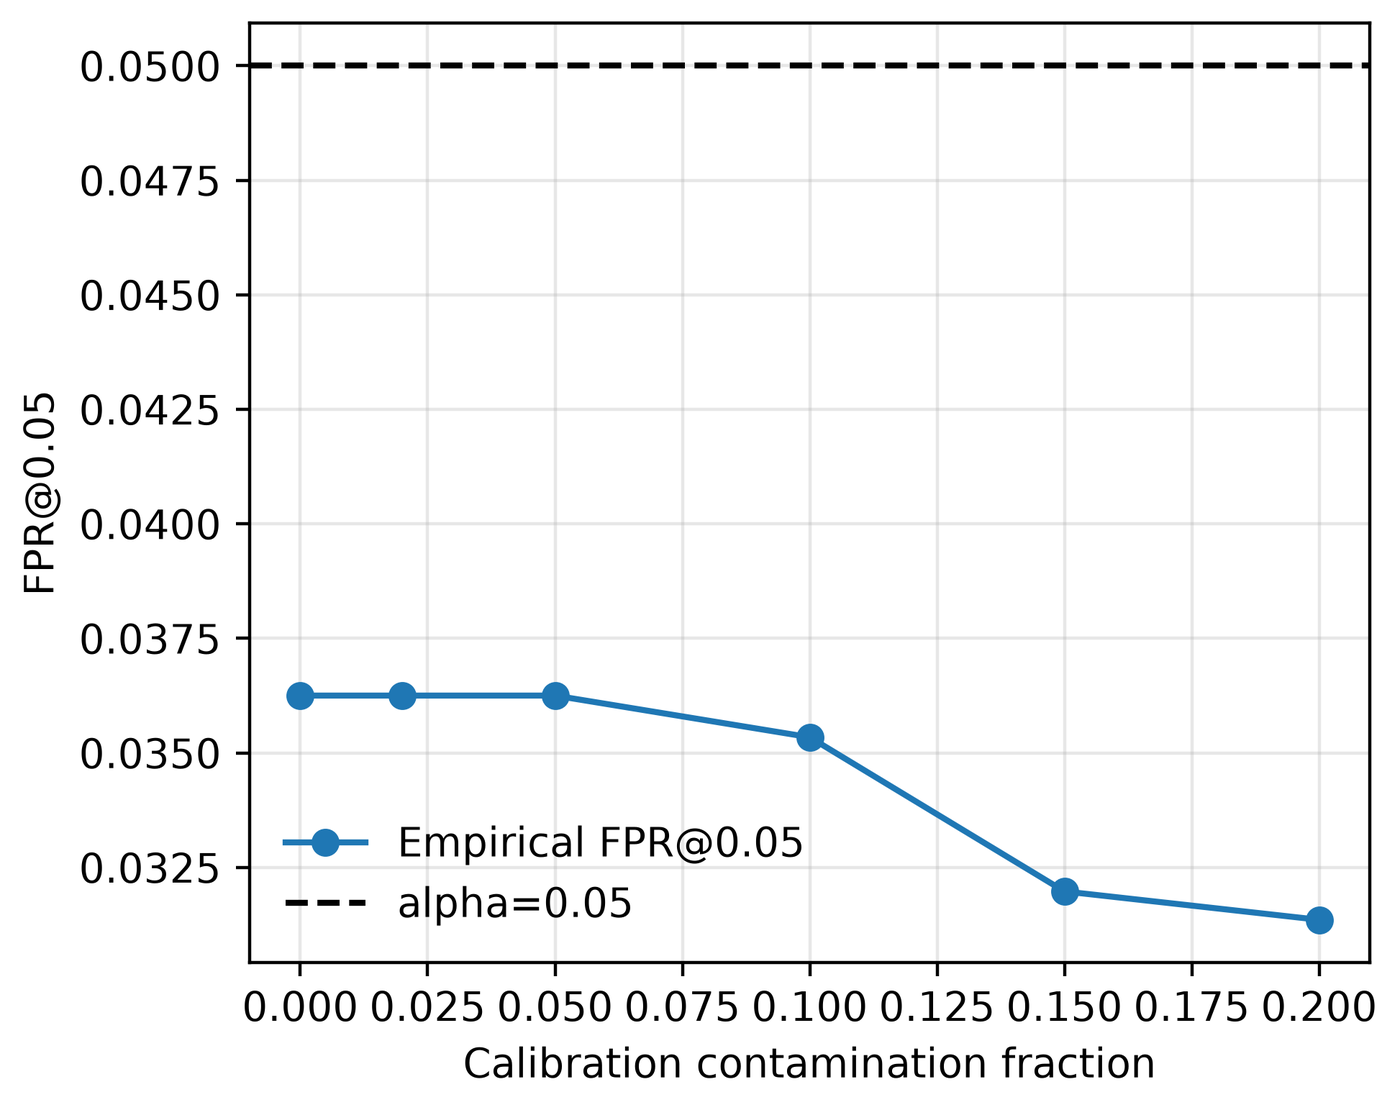
\includegraphics[width=0.85\linewidth]{figures/fig_contamination.png}
\caption{Calibration-set contamination on Cora ($\alpha=0.05$): empirical FPR among normal test nodes versus anomaly fraction $\pi_{\mathcal{C}}$ in the calibration set (from \texttt{results/studies.csv}).}
\label{fig:contamination}
\end{figure}

Table~\ref{tab:abl_contamination} shows FPR among normals \emph{decreases} as $\pi_{\mathcal{C}}$ increases---consistent with the score convention (higher $s$ = more anomalous) and Section~\ref{sec:th_limitations}. At $\pi_{\mathcal{C}}=0.20$ the conformal AUC collapses to $0.5$ because the contamination protocol moves so many anomalies into $\mathcal{C}$ that the test set retains too few positives for a meaningful ranking metric; FPR among remaining normals remains well-defined and continues the conservative trend. Extended multi-dataset contamination (Cora/Citeseer/PubMed, $\pi_{\mathcal{C}}$ up to $0.30$) is in Table~\ref{tab:contamination_multi}.

\begin{table}[pos=t]
\centering
\caption{Multi-dataset contamination: normal-node FPR@0.05 vs.\ $\pi_{\mathcal{C}}$ (mean$\pm$std, 5 seeds).}
\label{tab:contamination_multi}
\begin{tabular}{cccc}
\toprule
$\pi_{\mathcal{C}}$ & FPR (citeseer) & FPR (cora) & FPR (pubmed) \\
\midrule
0.00 & 0.039$\pm$0.012 & 0.034$\pm$0.012 & 0.039$\pm$0.005 \\
0.02 & 0.039$\pm$0.012 & 0.034$\pm$0.012 & 0.039$\pm$0.005 \\
0.05 & 0.039$\pm$0.012 & 0.034$\pm$0.012 & 0.039$\pm$0.005 \\
0.10 & 0.035$\pm$0.011 & 0.029$\pm$0.012 & 0.032$\pm$0.009 \\
0.15 & 0.032$\pm$0.009 & 0.026$\pm$0.012 & 0.029$\pm$0.010 \\
0.20 & 0.032$\pm$0.010 & 0.026$\pm$0.012 & 0.028$\pm$0.010 \\
0.25 & 0.032$\pm$0.010 & 0.026$\pm$0.012 & 0.028$\pm$0.010 \\
0.30 & 0.032$\pm$0.010 & 0.026$\pm$0.012 & 0.028$\pm$0.010 \\
\bottomrule
\end{tabular}

\end{table}

\subsubsection{Multiple Backbones under One Wrapper}
\label{sec:abl_backbones}

To substantiate the backbone-agnostic claim, we wrap scorers with the same CRC-GAD layer on Cora, Citeseer, and PubMed (seeds $\{0,\ldots,4\}$): simplified CoLA-inspired contrastive, \textbf{PyTorch DOMINANT} (shared GCN encoder + attribute/structure decoders following~\cite{ding2019dominant} and the authors' public PyTorch layout), a lighter NumPy DOMINANT-style reconstruction scorer, plus degree, feature-norm, and attribute-deviation heuristics (Table~\ref{tab:backbones}). The point is not that every backbone attains high AUC---several structural/attribute heuristics are weak by design---but that conformal FPR semantics attach to whatever score vector is supplied. Wall-clock scoring+calibration times are reported in the same table.

\begin{table*}[pos=t]
\centering
\caption{CRC-GAD on multiple backbones (mean$\pm$std over 5 seeds; $\alpha=0.05$). Generated from \texttt{results/extended\_studies.csv} and \texttt{results/dominant\_pytorch.csv}. Row \texttt{dominant} is a PyTorch reimplementation of Ding et al.\ (shared GCN encoder, attribute decoder, $A{=}ZZ^\top$ structure decoder); \texttt{dominant\_style} is the lighter NumPy reconstruction scorer.}
\label{tab:backbones}
\resizebox{\textwidth}{!}{%
\begin{tabular}{llccc}
\toprule
Backbone & Metric & Citeseer & Cora & Pubmed \\
\midrule
cola & Raw AUC & 0.759$\pm$0.006 & 0.691$\pm$0.024 & 0.735$\pm$0.034 \\
 & FPR@0.05 & 0.038$\pm$0.010 & 0.048$\pm$0.007 & 0.040$\pm$0.004 \\
 & TPR@0.05 & 0.230$\pm$0.089 & 0.110$\pm$0.063 & 0.166$\pm$0.019 \\
 & Time (s) & 4.158$\pm$0.048 & 1.641$\pm$0.020 & 7.730$\pm$0.274 \\
\midrule
dominant & Raw AUC & 0.687$\pm$0.008 & 0.676$\pm$0.017 & 0.926$\pm$0.002 \\
 & FPR@0.05 & 0.028$\pm$0.014 & 0.031$\pm$0.014 & 0.025$\pm$0.006 \\
 & TPR@0.05 & 0.444$\pm$0.081 & 0.486$\pm$0.126 & 0.532$\pm$0.024 \\
 & Time (s) & 18.425$\pm$2.395 & 6.945$\pm$0.556 & 270.285$\pm$43.727 \\
\midrule
conad & Raw AUC & 0.785$\pm$0.051 & 0.663$\pm$0.073 & --- \\
 & FPR@0.05 & 0.036$\pm$0.013 & 0.037$\pm$0.015 & --- \\
 & TPR@0.05 & 0.316$\pm$0.111 & 0.198$\pm$0.091 & --- \\
 & Time (s) & 108.257$\pm$9.043 & 36.300$\pm$1.882 & --- \\
\midrule
dominant\_style & Raw AUC & 0.213$\pm$0.015 & 0.203$\pm$0.019 & 0.664$\pm$0.004 \\
 & FPR@0.05 & 0.056$\pm$0.016 & 0.046$\pm$0.017 & 0.027$\pm$0.008 \\
 & TPR@0.05 & 0.005$\pm$0.011 & 0.006$\pm$0.013 & 0.515$\pm$0.012 \\
 & Time (s) & 8.927$\pm$2.621 & 2.204$\pm$0.350 & 22.740$\pm$4.648 \\
\midrule
degree & Raw AUC & 0.245$\pm$0.008 & 0.262$\pm$0.019 & 0.243$\pm$0.005 \\
 & FPR@0.05 & 0.043$\pm$0.013 & 0.041$\pm$0.013 & 0.050$\pm$0.005 \\
 & TPR@0.05 & 0.020$\pm$0.018 & 0.029$\pm$0.028 & 0.024$\pm$0.007 \\
 & Time (s) & 0.000$\pm$0.000 & 0.000$\pm$0.000 & 0.001$\pm$0.000 \\
\midrule
feature\_norm & Raw AUC & 0.257$\pm$0.015 & 0.248$\pm$0.018 & 0.748$\pm$0.004 \\
 & FPR@0.05 & 0.046$\pm$0.014 & 0.037$\pm$0.018 & 0.026$\pm$0.008 \\
 & TPR@0.05 & 0.037$\pm$0.012 & 0.006$\pm$0.013 & 0.520$\pm$0.012 \\
 & Time (s) & 0.085$\pm$0.004 & 0.023$\pm$0.001 & 0.065$\pm$0.001 \\
\midrule
attr\_deviation & Raw AUC & 0.274$\pm$0.014 & 0.281$\pm$0.020 & 0.659$\pm$0.005 \\
 & FPR@0.05 & 0.053$\pm$0.013 & 0.034$\pm$0.012 & 0.023$\pm$0.004 \\
 & TPR@0.05 & 0.010$\pm$0.013 & 0.006$\pm$0.013 & 0.492$\pm$0.011 \\
 & Time (s) & 0.184$\pm$0.009 & 0.051$\pm$0.001 & 0.176$\pm$0.002 \\
\bottomrule
\end{tabular}
}

\end{table*}

\subsubsection{Degree-Stratified FPR}
\label{sec:abl_degree}

Global FPR near $\alpha$ can coexist with quartile-level deviations (Table~\ref{tab:degree_fpr}), illustrating the gap between marginal and local behaviour.

\begin{table}[pos=t]
\centering
\caption{Normal-node FPR@0.05 by degree quartile on Cora (mean$\pm$std, 5 seeds).}
\label{tab:degree_fpr}
\begin{tabular}{lcc}
\toprule
Degree bin & FPR@0.05 & \#normals \\
\midrule
Q1\_low & 0.000$\pm$0.000 & 249.600$\pm$4.923 \\
Q2 & 0.004$\pm$0.003 & 140.200$\pm$11.356 \\
Q3 & 0.010$\pm$0.008 & 122.800$\pm$36.597 \\
Q4\_high & 0.154$\pm$0.071 & 138.400$\pm$21.360 \\
\bottomrule
\end{tabular}

\end{table}

\subsubsection{Organic Rare-Class Proxy}
\label{sec:abl_organic}

As a non-injected stress test, we mark the rarest Planetoid class on Cora as anomalous (\texttt{organic\_cora}). This is an \emph{organic class-imbalance proxy}, not a fraud label set. Table~\ref{tab:organic} reports CRC-GAD with several backbones under this definition.

\begin{table}[pos=t]
\centering
\caption{Organic rare-class proxy on Cora (mean$\pm$std, 5 seeds, $\alpha=0.05$).}
\label{tab:organic}
\footnotesize
\resizebox{\linewidth}{!}{\begin{tabular}{lcccccc}
\toprule
Backbone & \multicolumn{2}{c}{Citeseer} & \multicolumn{2}{c}{Cora} & \multicolumn{2}{c}{YelpChi} \\
\cmidrule(lr){2-3}\cmidrule(lr){4-5}\cmidrule(lr){6-7}
 & AUC & FPR & AUC & FPR & AUC & FPR \\
\midrule
attr.\ dev. & 0.506$\pm$0.000 & 0.042$\pm$0.007 & 0.473$\pm$0.000 & 0.059$\pm$0.009 & 0.587$\pm$0.000 & 0.043$\pm$0.001 \\
cola & 0.455$\pm$0.010 & 0.047$\pm$0.011 & 0.499$\pm$0.018 & 0.051$\pm$0.010 & --- & --- \\
degree & 0.549$\pm$0.007 & 0.035$\pm$0.010 & 0.512$\pm$0.004 & 0.040$\pm$0.006 & 0.530$\pm$0.000 & 0.044$\pm$0.002 \\
DOM-style & 0.461$\pm$0.006 & 0.061$\pm$0.009 & 0.466$\pm$0.006 & 0.058$\pm$0.015 & --- & --- \\
feat.\ norm & --- & --- & --- & --- & 0.539$\pm$0.000 & 0.046$\pm$0.002 \\
\bottomrule
\end{tabular}
}
\end{table}

\subsubsection{Comparison with Supervised Conformal Baseline}
\label{sec:abl_crcsgad}

Supervised conformal risk control with labeled anomalies~\cite{bates2023testing} is an \emph{orthogonal} setting (labels required). We do not claim CRC-GAD matches supervised power; our setting deliberately forgoes anomaly labels at calibration time.

\section{Conclusion and Future Work}
\label{sec:conclusion}

We studied unsupervised graph anomaly \emph{calibration}: how to turn frozen node scores into decisions at a nominal level $\alpha$ with an auditable finite-sample statement.
\textbf{CRC-GAD} does this by split conformal p-values under a label-free random partition.
It is a calibration protocol wrapped around existing scorers (including CoLA-style and DOMINANT), not a competitor claiming a new detection architecture.
The theorem we prove is \emph{marginal random-test-node validity} (Theorem~\ref{thm:randomization})---not node-conditional FPR, and not an automatic normal-node FPR bound without a ranking/dominance bridge.
When that bridge fails, empirical FPR can exceed $\alpha$; we report such cases rather than selecting only favourable graphs.

Empirically, the same wrapper applies to multiple scorers, heuristic comparisons extend beyond Cora, contamination and degree-stratified diagnostics quantify where the guarantee is fragile, and an organic rare-class proxy complements injected benchmarks.
All numbers regenerate from pinned code.

Limitations remain: CONAD under the identical protocol is left for future work; the organic proxy is not a real fraud graph; and concentration of single-deployment FPR is left empirical.
Future work includes trimmed calibration under contamination~\cite{bates2023testing}, online updates on evolving graphs, and tighter coupling to domain-specific review policies.
CRC-GAD is best read as a \emph{calibration protocol} for graph anomaly scores: a deployment layer with precise, limited guarantees, not universal risk control.


\section*{Declarations}

\noindent\textbf{Declaration of originality.} This manuscript reports original experimental results regenerated from the authors' pinned codebase. No numerical values were copied from previously published tables. Prior scorers and theory (in particular CoLA~\cite{liu2022cola}, DOMINANT~\cite{ding2019dominant}, and conformal prediction~\cite{vovk2005algorithmic,bates2023testing}) are cited as foundations; CRC-GAD claims only the calibration protocol and the associated analysis, not authorship of those components.

\noindent\textbf{Declaration of generative AI use.} Generative AI tools were used for manuscript editing, LaTeX formatting, and code-assistance during the reproducibility rebuild; all experiments, numerical results, and scientific claims were designed, executed, and verified by the authors.

\noindent\textbf{Declaration of competing interests.} The authors declare that they have no known competing financial interests or personal relationships that could have appeared to influence the work reported in this paper.

\noindent\textbf{Data and code availability.} Source code and scripts to reproduce all tables are at \url{https://github.com/Amaanullakhan/CRC_GAD} (tag \texttt{v1.0-rebuild}). Datasets (Cora, Citeseer, Pubmed, ACM, BlogCatalog, Flickr) are public benchmarks~\cite{ding2019dominant,liu2022cola}; download via \texttt{scripts/download\_datasets.py}. Anomaly injection and evaluation scripts are included.

\bibliographystyle{IEEEtran}
\bibliography{ref}

\end{document}
